\documentclass[a4paper,11pt]{article}
\usepackage[utf8]{inputenc}
\usepackage[T1]{fontenc}    % accents
\usepackage[english]{babel}
\usepackage[total={170mm,257mm}, left=20mm, top=20mm]{geometry}
\usepackage{parskip}   % Adds space between paragraphs instead of indentation
\usepackage{fancyhdr}  % For headers/footers

% Math & Fonts
\usepackage{amsmath}
\usepackage{amsfonts}
\usepackage{amssymb}
\usepackage{stmaryrd}  % For specific computer science math symbols
\usepackage{bbold}     % For blackboard bold numbers (e.g., indicator function)
\usepackage{newtxtext,newtxmath}

% Graphics & Visuals
\usepackage{graphicx}
\usepackage{float}       % For 'H' float option
\usepackage{subcaption}  % For side-by-side figures
\usepackage{tikz}
\usetikzlibrary{3d,calc,positioning}
\usepackage{placeins}    % For \FloatBarrier

% Algorithms & Utilities
\usepackage{algorithm}
\usepackage{algorithmic}
\usepackage{import}
\usepackage{url}
\usepackage{datetime}
\usepackage[hidelinks]{hyperref} % Makes TOC and References clickable

% Configurations
\graphicspath{{images/}}
\newcommand{\bfu}[1]{\textbf{\underline{#1}}}
\captionsetup[figure]{name={Fig.}, labelsep=period}
\usepackage[font=small,skip=5pt]{caption}

\date{Novembre 2025}

\begin{document}
\begin{titlepage}
    \centering
    \begin{minipage}{0.45\textwidth}
        \begin{flushleft}
            
\includegraphics[height=2cm]{image_n7.png}
        \end{flushleft}
    \end{minipage}
    \hfill
    \begin{minipage}{0.45\textwidth}
        \begin{flushright}
            
\includegraphics[height=2.3cm, trim=0 290 0 290, clip]{1200px-Logo_INSAvilletoulouse-RVB-carre.jpg}
        \end{flushright}
    \end{minipage}

    \vspace{2cm}

    {\Large ModIA 2\textsuperscript{nd} Year Project Report}

    \vfill
    { \huge \bfseries Use of Hawkes processes in a \\[0.3cm] Cramér-Lundberg type model \par}
    \vfill

    \begin{minipage}[t]{0.45\textwidth}
        \begin{flushleft} \large
            \textit{Authors}\\
            Driss \textsc{Chraibi}\\
            Wassim \textsc{Fathi}\\
            Paul \textsc{Louka}
        \end{flushleft}
    \end{minipage}
    \hfill
    \begin{minipage}[t]{0.45\textwidth}
        \begin{flushright} \large
            \textit{Supervisors}\\
            Prof. Mélisande \textsc{Albert}\\
            Prof. Anthony \textsc{Réveillac}\\
            Prof. Rebecca \textsc{Coles}
        \end{flushright}
    \end{minipage}

    \vfill
    {\large Academic Year 2025--2026}
\end{titlepage}

\clearpage

\renewcommand{\contentsname}{Table of Contents}
\tableofcontents

\clearpage

\listoffigures
\clearpage 

\section*{Introduction}
\addcontentsline{toc}{section}{Introduction}

For an insurance company, the main goal is to accurately model the risk of ruin associated with claim occurrences and sizes. Doing so enables the company to set appropriate premiums, maintain sufficient reserves, and ensure long-term profitability, i.e.,
a growing surplus. 

Claim occurences can be modeled using counting or point processes, which represent the number of events occurring over time. One of the simplest point processes is the well studied homogeneous Poisson process, which assumes that events occur independently and at a constant average rate, also known as intensity. This is a reasonable model for phenomena such as the arrival of calls at a call center. By allowing the intensity to vary, it is possible to extend to the inhomogeneous case, which makes it possible to capture time-dependent patterns such as rush-hour traffic.

However, both models assume that the number of events in one period does not affect the number of events in another period. This assumption does not hold for events like earthquakes, epidemic spreads, or market crashes, where a main shock often causes a sequence of aftershocks. In insurance, claim occurrences also exhibit clustering behavior, where one claim can increase the likelihood of subsequent claims. To capture this phenomenon, we used the Hawkes process, which is a self-exciting model capable of capturing these effects.

The aim of the study is to simulate the Hawkes process and quantify how the clustering of events affects the surplus. Our approach relies on Ogata’s thinning algorithm, a simulation technique based on rejection sampling used to generate point processes with time-dependent intensities.

In Sections 1 and 2, we approach the problem theoretically by defining the mathematical framework, characterizing the exponential kernel, and deriving the mean intensity. In Section 3, we analyze the expected number of claims, establishing the net profit condition (NPC) to ensure that the collected premiums are sufficient to cover the expected claim load. In Section 4, we implement Ogata's thinning algorithm to simulate the Hawkes process and analyze how the kernel parameters influence the clustering behavior of claims. In Section 5, we quantify the effect of clustering on the probability of ruin. Using a Monte Carlo approach, we compute the probability of ruin for different values of initial capital and premium rates. We also evaluate the model’s robustness by analyzing parameter estimation errors and propose risk mitigation strategies.

\clearpage
\section{Mathematical Background and Notations}

\subsection{Counting Processes and Filtration}
We consider a probability space $(\Omega, \mathcal{F}, \mathbb{P})$. To model the arrival of insurance claims, we utilize a counting process $N = (N(t))_{t \geq 0}$.

\textbf{Definition 1.} A counting process is a sequence of random variables such that:
\begin{enumerate}
    \item[(i)] $N(0) = 0$ and $N(t)$ takes values in $\mathbb{N}$ for all $t \geq 0$;
    \item[(ii)] The paths $t \mapsto N(t)$ are non-decreasing and right-continuous.
\end{enumerate}

The claim arrival times are denoted by the strictly increasing sequence of random variables $ (T_k)_{k \geq 1}$.

\subsection{Poisson Processes}
The Poisson process is a well studied counting process, commonly used to model arrival times of random events. As mentioned in the introduction, we distinguish between two cases: homogeneous and inhomogeneous Poisson processes.

\textbf{Definition 2.} A counting process $N$ is a homogeneous Poisson process with rate $\lambda > 0$ if:
\begin{enumerate}
    \item[(i)] It has independent increments;
    \item[(ii)] The number of events in any interval $(s, t]$ follows a Poisson distribution with parameter $\lambda(t-s)$.
\end{enumerate}

\textbf{Definition 3.} A counting process $N$ is an inhomogeneous Poisson process with intensity function $\lambda(t) \ge 0$ if:
\begin{enumerate}
    \item[(i)] It has independent increments;
    \item[(ii)] The number of events in any interval $(s, t]$ follows a Poisson distribution with parameter $\int_s^t \lambda(u) du$.
\end{enumerate}

\subsection{Conditional Intensity Function}
To extend these definitions to self-exciting models, we utilize the conditional intensity function $\lambda(t)$. Intuitively, $\lambda(t)dt$ represents the probability of an event occurring in the infinitesimal interval $[t, t+dt)$ given the full history of the process up to time $t$. Formally, this history corresponds to the natural filtration $\mathcal{F}_t = \sigma(N(s), s \le t)$.

Thus the stochastic intensity is defined as:
\begin{equation}
    \lambda(t|\mathcal{F}_t) = \lim_{h \to 0^+} \frac{\mathbb{P}(N(t+h) - N(t) = 1 | \mathcal{F}_t)}{h}
\end{equation}

This definition highlights the key difference between the models:
\begin{enumerate}
    \item[(i)] For a Poisson process (homogeneous or inhomogeneous), the intensity is deterministic and independent of the history $\mathcal{F}_t$.
    \item[(ii)] For a self-exciting process, the intensity is a stochastic process adapted to $\mathcal{F}_t$. It explicitly depends on the timing of previous events $T_k < t$.
\end{enumerate}

\subsection{The Cramér-Lundberg Risk Model}
We formally define the insurer's surplus process $R(t)$ as:
\begin{equation}
    R(t) = u + ct - S(t)
\end{equation}
where $u \ge 0$ is the initial capital, and $c > 0$ is the constant premium rate.\\ The aggregate claim amount $S(t)$ is defined by:
\begin{equation}
    S(t) = \sum_{i=1}^{N(t)} X_i
\end{equation}
Here, $N(t)$ represents the number of claims up to time $t$, modeled as a Poisson process, and $X_i$ are i.i.d. non-negative random variables representing claim sizes. We assume the sequence $(X_i)$ is independent of the process $N(t)$.

As an insurance company, the primary objective is to analyze the probability of ruin, defined as:
\begin{equation}
    \psi(u) = \mathbb{P}(\exists t \ge 0 : R(t) < 0 | R(0) = u)
\end{equation}
This probability quantifies the risk that the insurer's surplus becomes negative at some point in time, i.e. that the company goes bankrupt.


\section{Hawkes Process}
\subsection{Poisson Process Limitations}

The homogeneous Poisson process relies on two strong assumptions: independent increments and the stationarity of the intensity $\lambda(t)$. While the inhomogeneous extension allows the intensity to vary deterministically with time, it remains independent of $\mathcal{F}_t$.

However, this modeling approach fails whenever the observed phenomenon has self-exciting properties (where an event temporarily increases the likelihood of the next claim). In fields such as seismology or actuarial science, such a model becomes inadequate, as it underestimates the risk of contagion.

\subsection{Definition of the Hawkes Process}

A. G. Hawkes introduced self-exciting processes to model dynamics where contagion is non-negligible \cite{hawkes1974}.

Let $N_{hawkes} = (N_{hawkes}(t))_{t \geq 0}$ be a counting Hawkes process representing the number of claims up to time $t$, and let $ (T_k)_{k \geq 1}$ denote the ordered arrival times.

The conditional intensity function of $N_{hawkes}$ is defined as
$$
\lambda(t) = \mu + \int_0^t \phi(t - s) dN_{hawkes}(s) = \mu + \sum_{t_k < t} \phi(t - t_k),
$$
where $\mu > 0$ is the baseline intensity and $\phi \in L^1(\mathbb{R}_+)$ is the excitation function or kernel \cite{bacry2015}.

\subsection{Exponential Kernel}

From now on, we consider the exponential kernel defined as $\phi(t) = \alpha e^{-\beta t}$ with parameters $\alpha, \beta > 0$.

$\alpha$ is know as the excitation parameter, it represents the instantaneous increase in intensity caused by a claim. $\beta$ is the decay parameter, which controls the rate at which the intensity decreases towards its baseline level $\mu$.

The influence of a claim is maximal ($\alpha$) at the instant of its occurrence, then decays exponentially at a rate $\beta$.
The intensity function can be expressed as
$$\lambda(t) = \mu + \sum_{T_k < t} \alpha e^{-\beta(t - T_k)}$$

Furthermore, as established by Hawkes \cite{hawkes1974} in his cluster representation, the integral of the kernel over $[0, +\infty[$ corresponds to the average number of claims generated by a single excitation. This quantity is referred to as the branching ratio, denoted by $n$:
$$n = ||\phi||_1 = \int_0^{+\infty} \alpha e^{-\beta t} \, dt =\frac{\alpha}{\beta}
$$

Intuitively, to ensure stability and avoid divergence through chain reactions, an event must generate, on average, less than one direct descendant. Thus, we require the condition $n < 1$, or equivalently $\alpha < \beta$. We confirm this intuition in Section 3 by calculating the expected number of claims.


\clearpage
\section{Analysis of the Expected Number of Claims}

The introduction of self-excitation temporarily increases the intensity $\lambda(t)$ after each claim. Due to this dependency on the history of claims, the intensity $\lambda(t)$ becomes a stochastic process rather than a deterministic function. We aim to derive and analyze the exact expression of its expectation in Section 3.1.

\subsection{Expression of the Expectation}

We recall that the intensity function is
$$\lambda(t) = \mu + \sum_{T_k < t} \alpha e^{-\beta(t - T_k)}$$

The expectation of the counting process is given by the fundamental relation
$$\mathbb{E}[N_{hawkes}(t)] = \mathbb{E}\left[\int_0^t \lambda(s) ds\right]$$

Solving via Laplace transform as shown in Appendix A, we obtain the following expression for all $t \ge 0$:
$$\boxed{\mathbf{E}[N_{hawkes}(t)] = \frac{\mu}{\beta - \alpha} \left( \beta t - \frac{\alpha}{\beta - \alpha} (1 - e^{-(\beta - \alpha) t}) \right)}$$

We recover the condition $\alpha < \beta$ which ensures system stability. Otherwise, the exponential term $e^{-(\beta - \alpha) t}$ would diverge, leaving the system unstable.

\subsection{Asymptotic Analysis}
Let us examine the behavior as $t \to +\infty$.
 Since $\alpha < \beta$, the exponential term vanishes
$$e^{-(\beta - \alpha) t} \to 0$$
The expression then simplifies into two terms: a linear term in $t$ and a constant that is negligible compared to $t$
$$
\mathbf{E}[N_{hawkes}(t)] \sim \frac{\mu \beta}{\beta - \alpha} t - \frac{\mu \alpha}{(\beta - \alpha)^2}
$$

The linear term dominates and we obtain the following approximation:
$$
\boxed{\mathbf{E}[N_{hawkes}(t)] \sim \mu t*\frac{1 }{1 - n} \quad \text{when } t \to +\infty}
$$

This asymptotic expression of the expectation value validates the cluster representation proposed by Hawkes \cite{hawkes1974}. The counting process is split into independent families of events.

We distinguish two categories of events over the observation $[0, t]$ :
\begin{itemize}
    \item Immigrants (generation 0), arriving according to a Poisson process with intensity $\mu$. Their expected number is $\mu*t$
    \item Descendants (generations $1, 2, \dots$) arriving according to the self-excitation of the model.
\end{itemize}

Recall that $n$ represent the average number of direct events generated by a single excitation. Consequently, an event of generation $k$ generates, on average, $n$ events of generation $k+1$. We prove in Appendix B that an immigrant generates on average $n^k$ descendants at generation $k$. The expected size of a family (cluster) is therefore given by the sum of the geometric series

\begin{equation}
    \mathbb{E}[\text{Cluster size}] =\sum_{k=0}^{+\infty} \mathbb{E}[\text{Descendants generated at generation k}]   = \sum_{k=0}^{+\infty} n^k=\frac{1}{1-n}
\end{equation}

Thus, the expected total number of events for large $t$ is obtained by multiplying the average number of immigrants by the average cluster size
\begin{equation}
    \mathbb{E}[H_t] \approx \underbrace{\mu t}_{\text{Immigrants}} \times \underbrace{\frac{1}{1-n}}_{\text{Cluster size}}
\end{equation}

\subsection{Net Profit Condition}

The net profit condition (NPC) is the condition that the average capital inflow exceeds the average outflow in the long term. If this condition is not satisfied, the probability of ruin is equal to 1.

We recall the Cramér-Lundberg model:
$$R(t) = u + \underbrace{c \cdot t}_{\text{Cumulative gains}} - \underbrace{\sum_{i=1}^{N_{hawkes}(t)} X_i}_{\text{Cumulative losses}}$$

The premiums collected over a period $t$ must, on average, cover the total cost of claims during this period. Thus, we seek a condition such that
$$ \text{Cumulative gains} > \mathbb{E}[\text{Cumulative losses}]$$
$$ c \cdot t > \mathbb{E}\left[\sum_{i=1}^{N_{hawkes}(t)} X_i\right]$$
Using Wald's identity and the independence between $N_{hawkes}(t)$ and the claim sizes $X_i$, we have
$$ c \cdot t > \mathbb{E}[N_{hawkes}(t)] \cdot \mathbb{E}[X_1]$$

To establish a time-independent condition, we consider the asymptotic behaviour:
$$ c > \lim_{t \to +\infty} \frac{\mathbb{E}[N_{hawkes}(t)]}{t} \cdot \mathbb{E}[X_1] $$

Which finally leads to the net profit condition:
$$\boxed{c > \frac{\mu}{1-n} \cdot \mathbb{E}[X_1]}$$

However, the NPC only guarantees profitability in terms of expected value over an infinite horizon. It does not account for the variance and the temporal clustering of claims. Even if $c$ satisfies the condition, the high volatility during any given cluster may still lead to ruin in the short term. We investigate this possibility in the next section.


\clearpage
\section{Simulation and Numerical Analysis of Clustering}

While Section 3 established the theoretical stability conditions of the Hawkes process, analytical formulas for the distribution of aggregate claims are difficult to derive. To understand the risk of ruin, we must rely on Monte Carlo simulations.

However, unlike the Poisson process, the Hawkes intensity $\lambda(t)$ is stochastic and path-dependent. We cannot simply simulate independent inter-arrival times (as in the usual Poisson case). Instead, we must generate the entire path of the intensity function alongside the event times. In this section, we present the simulation methodology and analyze the specific impact of the kernel parameters on the risk profile.

\subsection{Ogata's Thinning Algorithm}
To simulate the process exacty, we implemented Ogata's Thinning Algorithm \cite{ogata1981}. This method relies on the acceptance-rejection principle adapted for point processes. The core idea is to generate candidate points using a homogeneous Poisson process with rate $\lambda^*$ s.t. $\lambda^* \ge \lambda(t)$. A candidate point at time $t$ is then accepted with probability $\frac{\lambda(t)}{\lambda^*}$.

Since we use an exponential kernel $\phi(t) = \alpha e^{-\beta t}$, the intensity strictly decays between jumps. Therefore, right after an event at time $T_k$, the intensity is maximal for the subsequent interval. We can thus update the upper bound as $\lambda^* = \lambda(T_k^+)$ after each accepted event. The procedure is detailed in Algorithm \ref{alg:ogata}.

\begin{algorithm}[H]
\caption{Ogata's Thinning Algorithm, adapted for Hawkes process with exponential kernel}
\label{alg:ogata}
\begin{algorithmic}[1]
\REQUIRE Parameters $\mu, \alpha, \beta, T$
\STATE Initialize $t \leftarrow 0$, $\mathcal{T} \leftarrow \emptyset$
\STATE Initialize bound $\lambda^* \leftarrow \mu$
\WHILE{$t < T$}
    \STATE Generate waiting time $S \sim \mathcal{E}(\lambda^*)$
    \STATE Update time $t \leftarrow t + S$
    \IF{$t > T$} \STATE Break \ENDIF
    \STATE Calculate intensity $\lambda(t) = \mu + \sum_{t_i \in \mathcal{H}} \alpha e^{-\beta(t - t_i)}$
    \STATE Generate $U \sim \mathcal{U}[0, 1]$
    \IF{$U \le \lambda(t) / \lambda^*$}
        \STATE $\mathcal{T}$ = $\mathcal{T} \cup \{t\}$ \hfill \COMMENT{Accept event}
        \STATE Update bound $\lambda^* \leftarrow \lambda(t) + \alpha$
    \ELSE
        \STATE Update bound $\lambda^* \leftarrow \lambda(t)$ \hfill \COMMENT{Reject event, intensity decays}
    \ENDIF
\ENDWHILE
\RETURN $\mathcal{T}$
\end{algorithmic}
\end{algorithm}

\subsection{Influence of Kernel Parameters $\alpha$ and $\beta$}
The behavior of the Hawkes process is directly tied to the branching ratio $n = \alpha / \beta$. However, two processes can have the same stability index $n$ but exhibit vastly different risk profiles depending on the magnitude of $\alpha$ and $\beta$.

Figure \ref{fig:intensity_influence} compares two regimes with the same branching ratio $n=0.8$:
\begin{itemize}
    \item High $\alpha$, High $\beta$: The intensity spikes violently after an event but returns to the baseline quickly. This models risks like chain-reaction accidents where the danger is immediate but on a short timescale.
    \item Low $\alpha$, Low $\beta$: The intensity rises less sharply but decays slowly. This models more persistent risks, such as an epidemic or a flood season, where the danger remains elevated for a long period.
\end{itemize}

\begin{figure}[H]
    \centering
    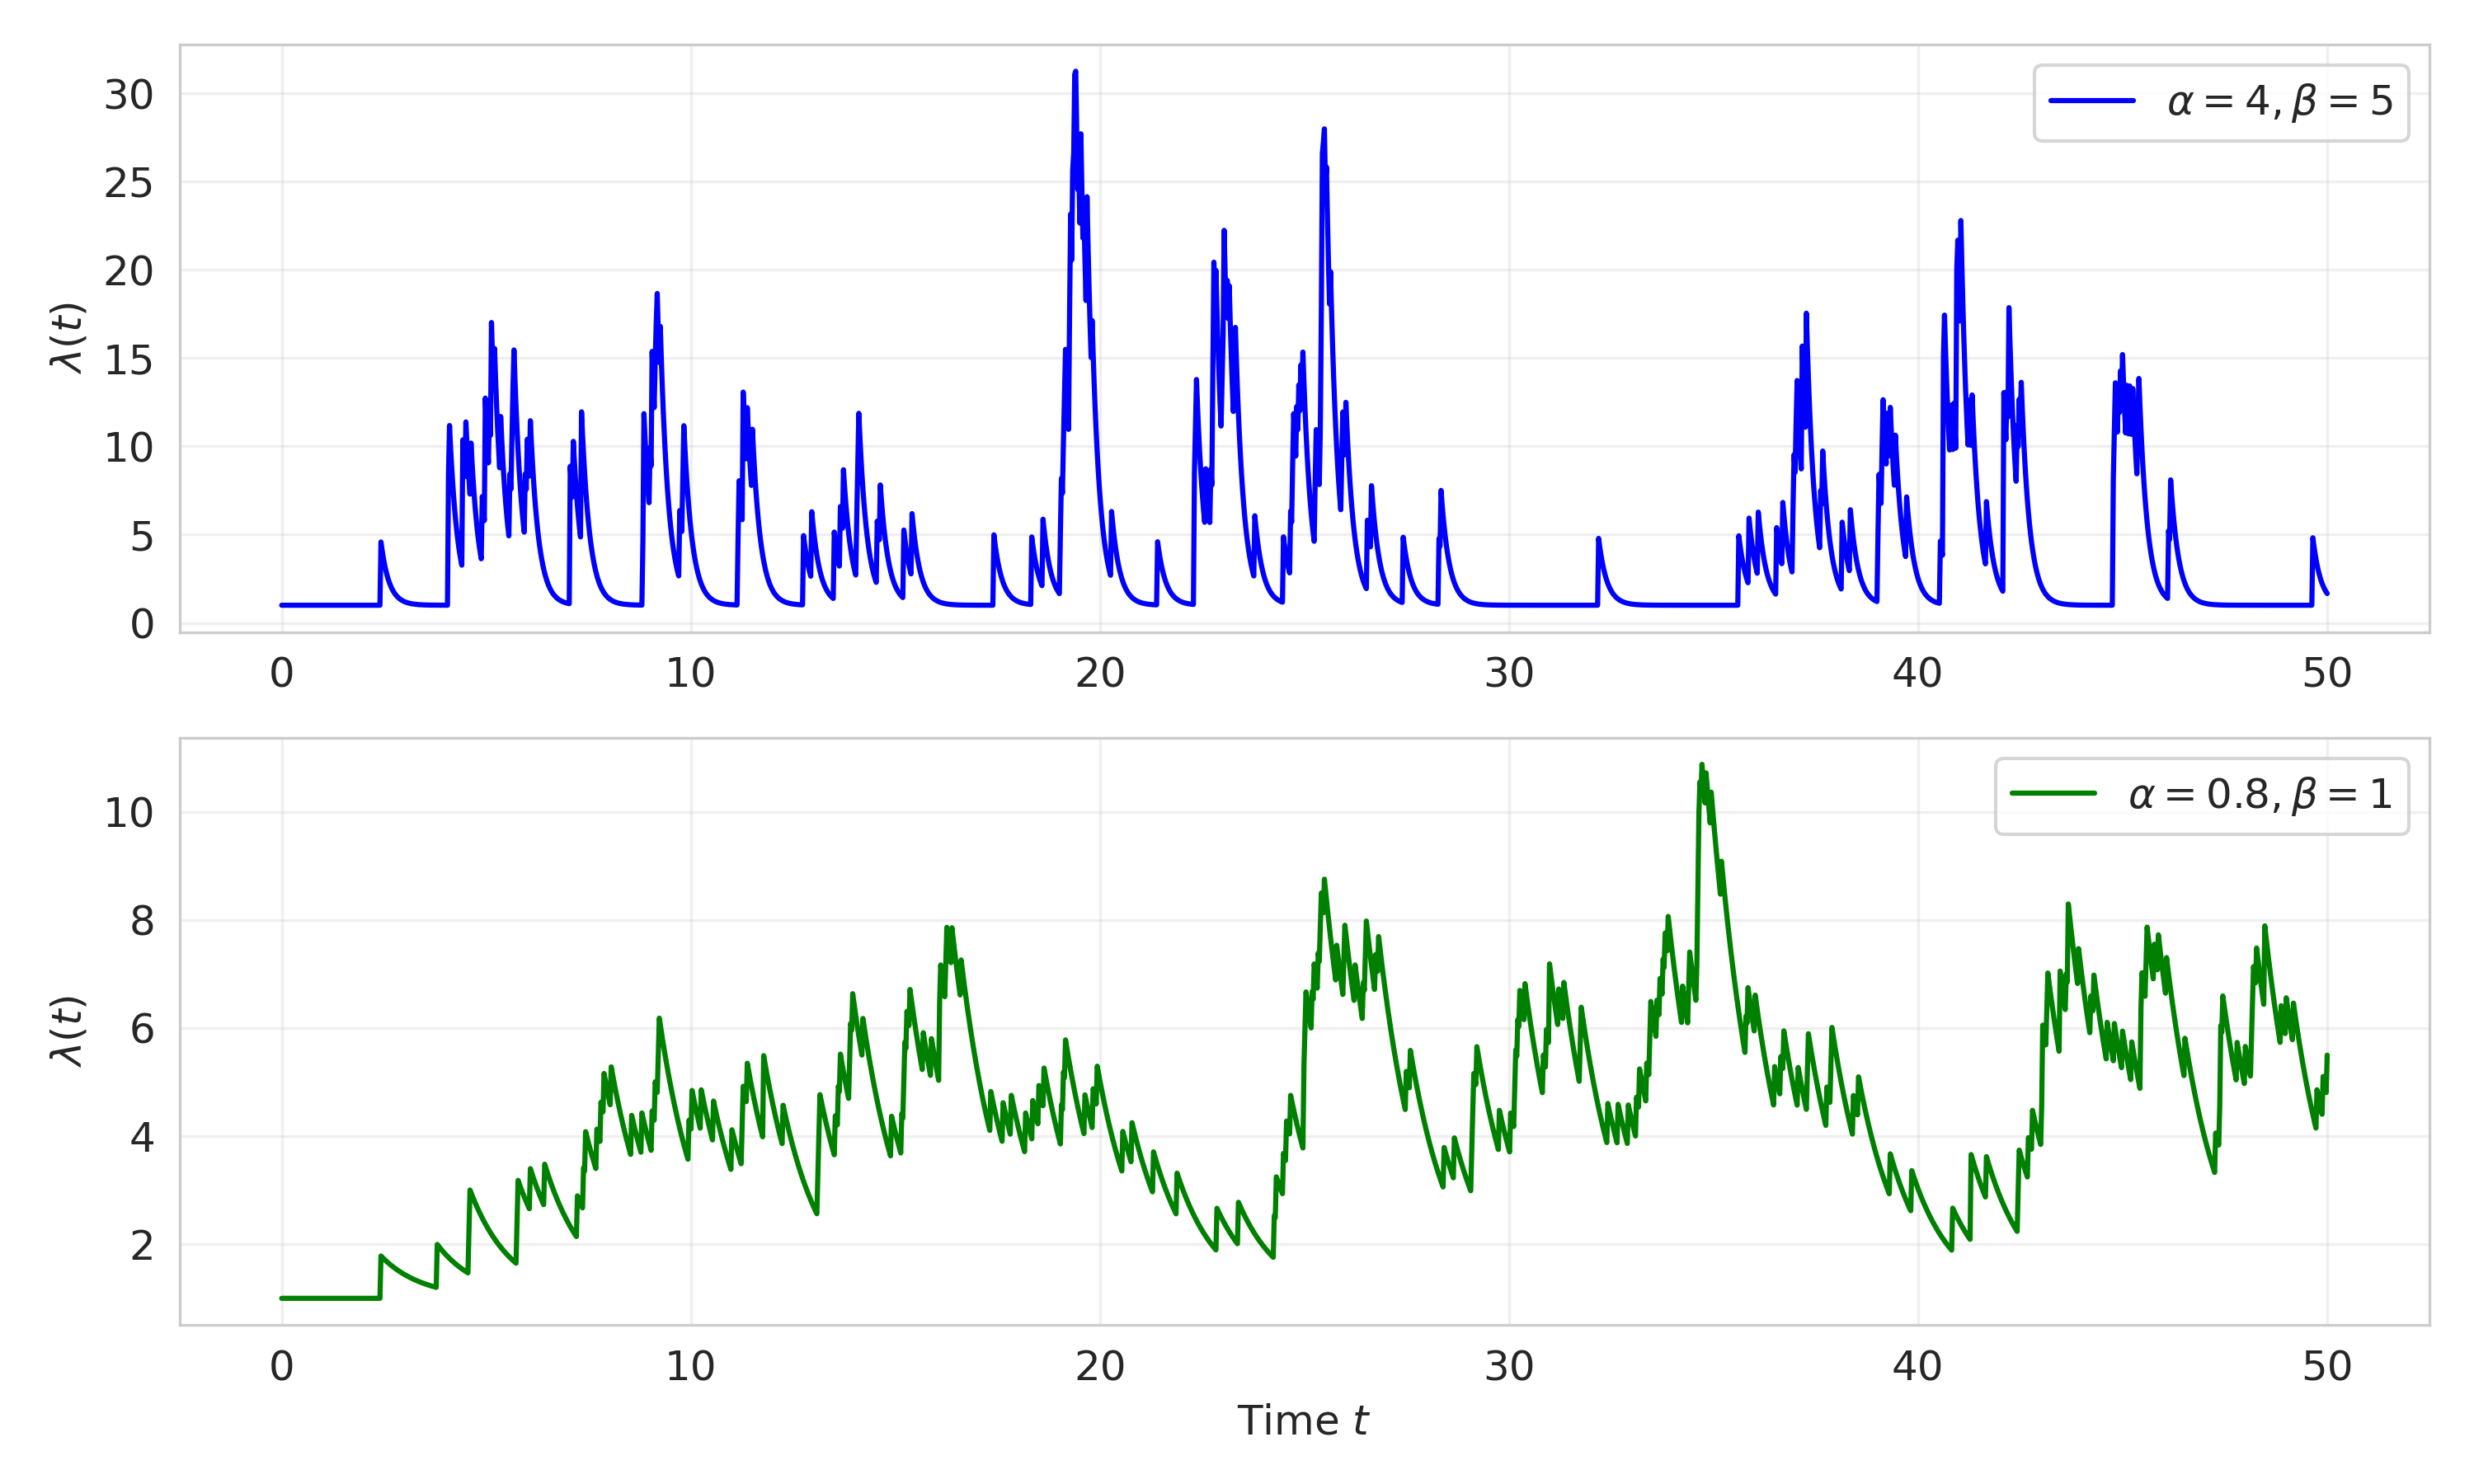
\includegraphics[width=0.65\textwidth]{images/intensity_influence.png}
    \caption{\textbf{Impact of kernel parameters on intensity dynamics.} Both processes share the same branching ratio $n=0.8$ and baseline $\mu=1.0$. \text{Left:} High excitation ($\alpha=4.0$) and fast decay ($\beta=5.0$) lead to sharp intensity spikes that quickly return to baseline. \text{Right:} Low excitation ($\alpha=0.4$) and slow decay ($\beta=0.5$) produce smaller increases but prolonged elevated intensity levels.
    } \label{fig:intensity_influence}

\end{figure}
\vspace{-1em}
In summary, while the branching ratio $n$ governs the average number of events generated per claim, the individual parameters $\alpha$ and $\beta$ shape the temporal clustering behavior. As seen here, a small $\beta$ leads to a long-memory effect: the impact of an event persists in the system. High $\alpha$ leads to more extreme spikes in intensity. Both effects can significantly influence the risk of ruin, as we explore further in Section 5.

\subsection{Clustering Effect on the Distribution of Claims}
The primary danger of the Hawkes process for insurers is not necessarily the average number of claims, but their variance. To quantify this, we simulated $2000$ trajectories of a Hawkes process and a Poisson process, both calibrated to have the exact same expected number of claims $\mathbb{E}[N(T)] = 250$.

As shown in Figure \ref{fig:clustering_hist}, while the means align, the distributions are highly different. The Hawkes process (in red) exhibits a significantly wider distribution with heavier tails (especially the right tail, i.e. higher counts) compared to the Poisson process (in blue).

\begin{figure}[H]
    \centering
    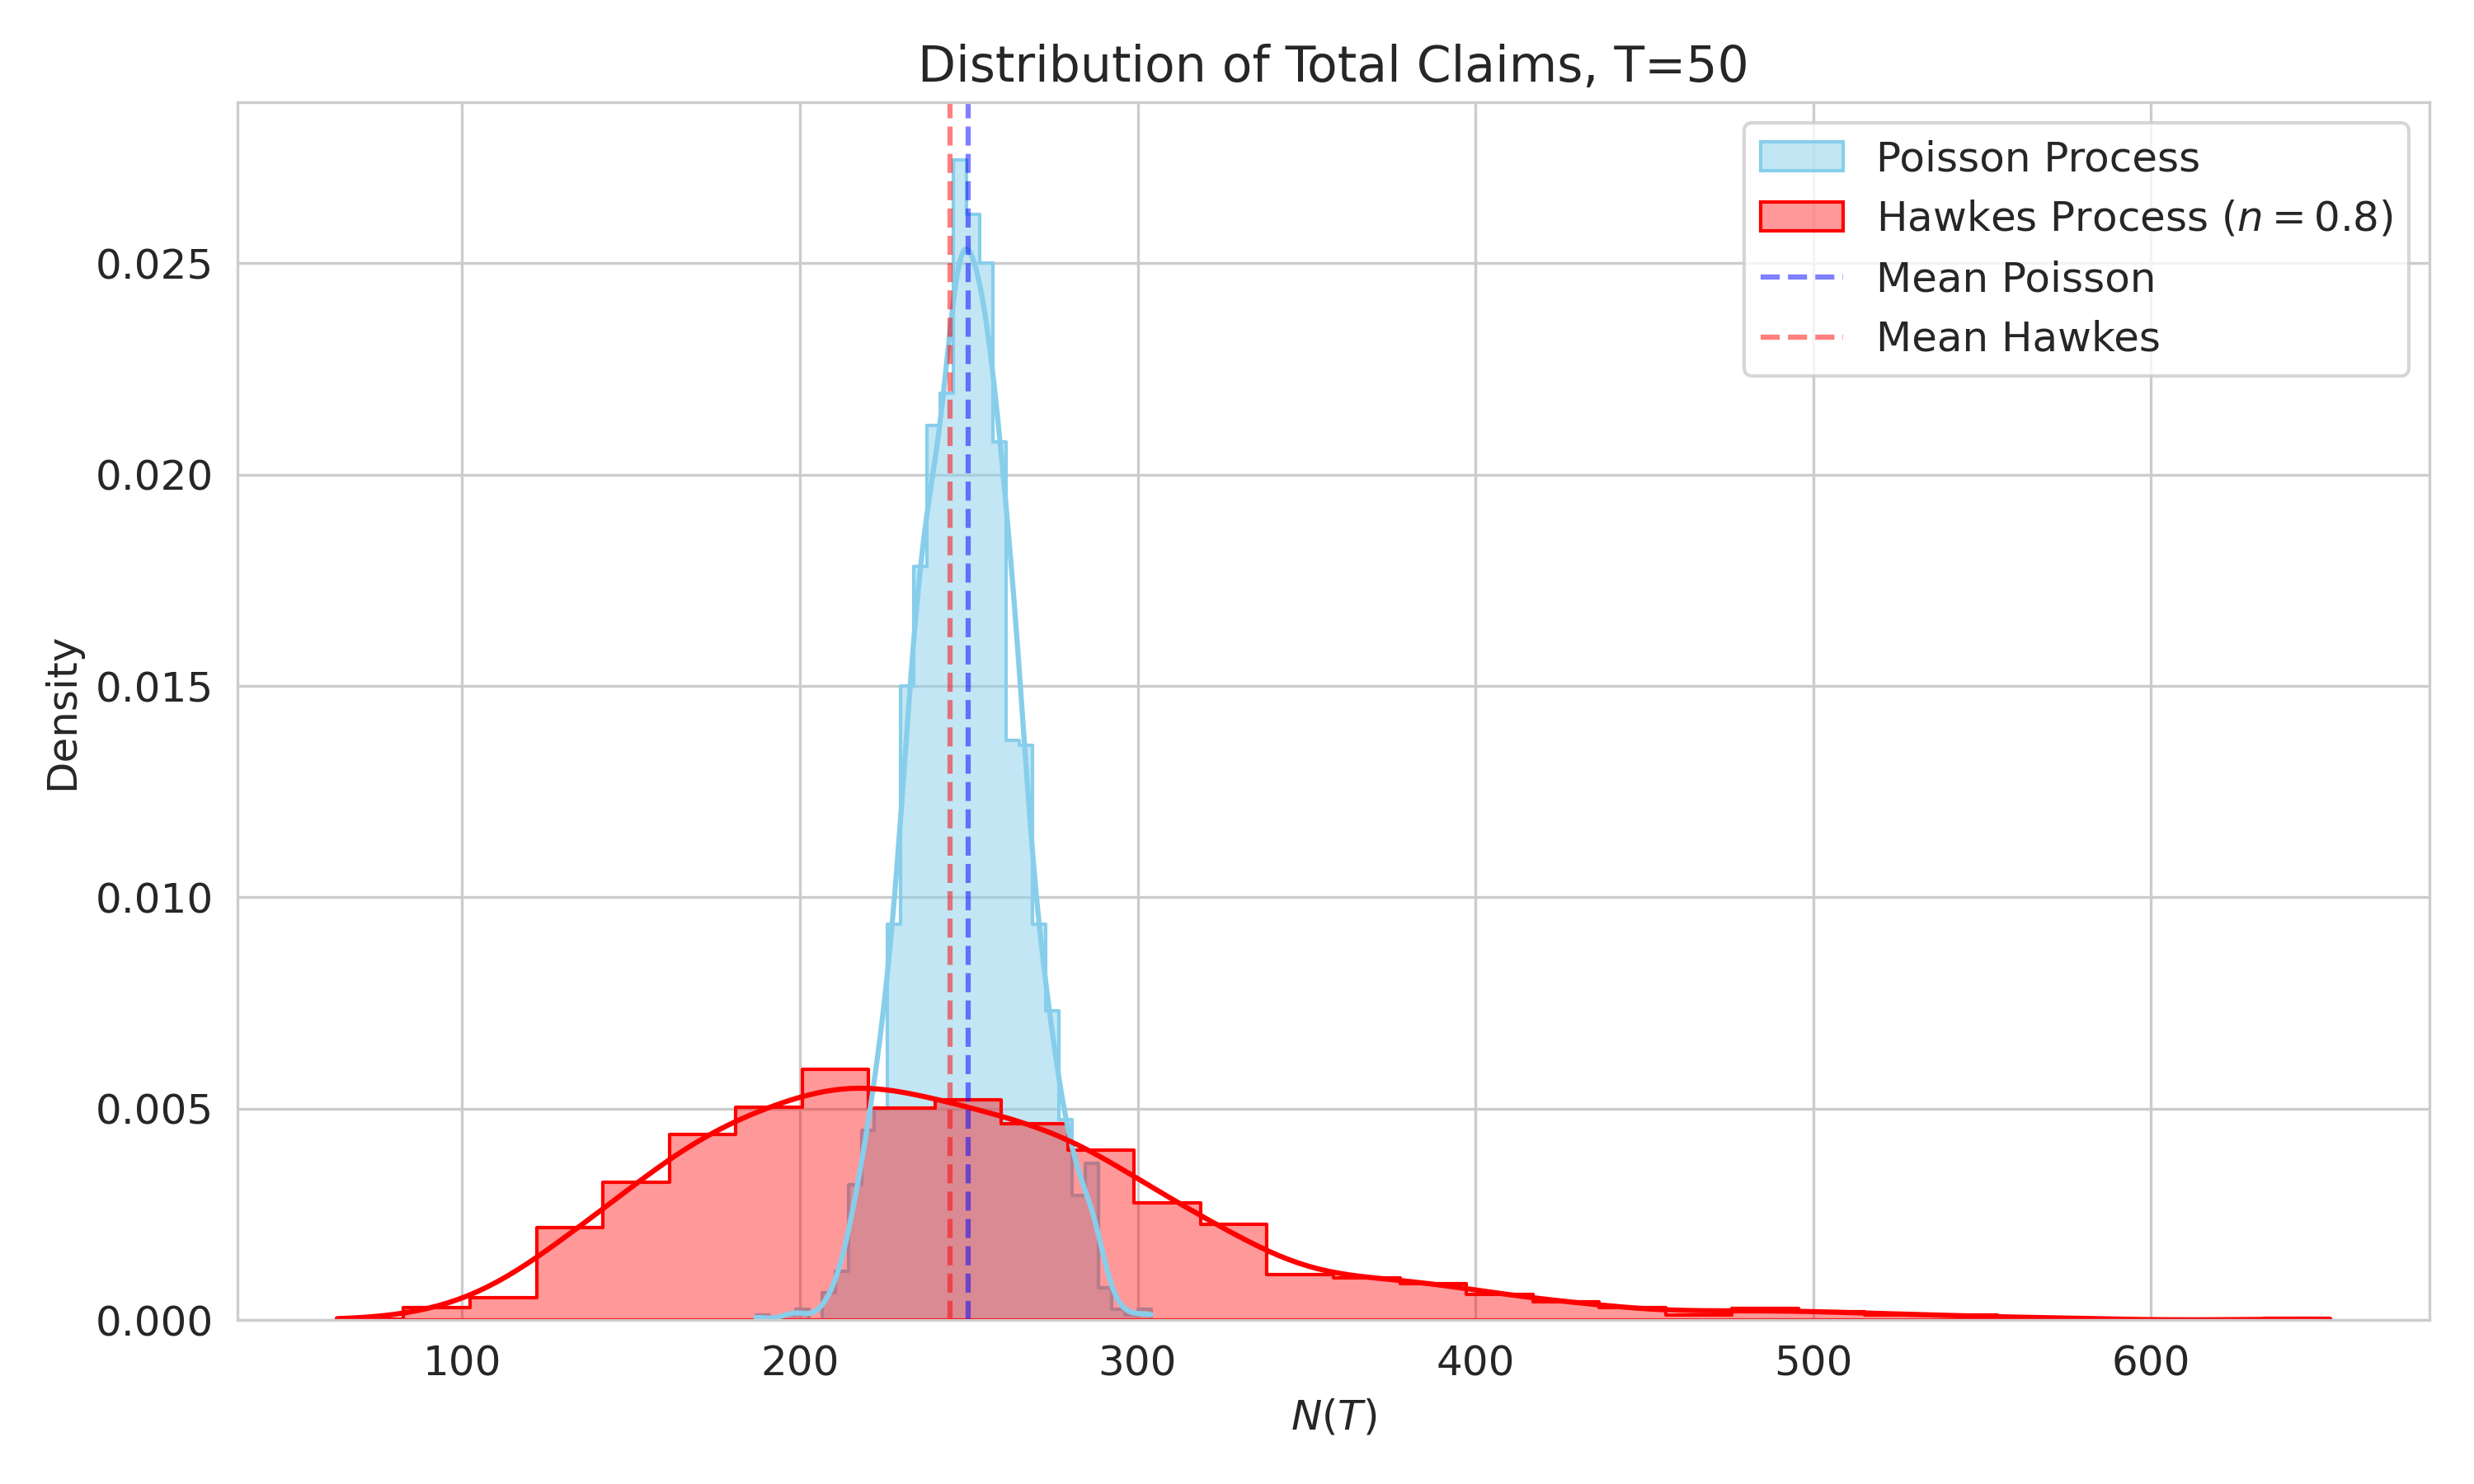
\includegraphics[width=0.65\textwidth]{images/clustering_histogram.png}
    \caption{\textbf{Distribution of claim counts ($T=50$).} The Hawkes process (red) shows a wider distribution compared to the Poisson reference, despite having the same theoretical mean. This indicates a higher probability of extreme claim volumes for the Hawkes case.}
    \label{fig:clustering_hist}
\end{figure}
\vspace{-1em}
These results show that for a premium calculated on the NPC, a Hawkes based portfolio faces a much higher probability of extreme losses than a Poisson based one. This statistical reality is the driver behind the ruin probabilities analyzed in the next section.

\clearpage
\section{Impact of the Clustering Effect on the Risk of Ruin}

\subsection{Simulation Framework}

We simulate three distinct risk processes with the same mean intensity to validate the dynamics of the intensity function $\lambda(t)$:

\begin{itemize}
    \item \textbf{Homogeneous Poisson Process (HPP):} 
    Serves as our stationary benchmark with a constant intensity $\lambda = 4.0$. 
    This implies that the expected counting process increases linearly over time ($\mathbb{E}[N(t)] = \lambda t$), representing a stable risk with independent increments.
    \item \textbf{Inhomogeneous Poisson Process (IPP):} 
    Captures deterministic seasonality (e.g., cyclic claim frequencies). 
    We modeled the intensity as $\lambda(t) = 4.0 + 2\sin(t)$. 
    Crucially, over full periods, the time-averaged intensity remains $\bar{\lambda} = 4.0$. This ensures expected number of claims matches the HPP benchmark, while introducing periodic volatility.
    \item \textbf{Hawkes Process:} 
    Incorporates the clustering effect where every event excites the intensity. 
    To maintain a fair comparison with the Poisson models (same global mean intensity $\mathbb{E}[\lambda_{\infty}] = 4.0$), we calibrated the baseline intensity $\mu$ according to the branching ratio ($n=0.75$) using the stationarity condition. This branching ratio means that each event generates, on average $n=0.75$ direct offspring. 
    This calibration ensures that the expected number of events is identical for both processes at any time horizon $t$.
    Substituting our calibration $\mu = \lambda (1-n) = 1.0$:
    $$ \mathbb{E}[N_{\text{Hawkes}}(t)] = \frac{\lambda (1-n)}{1-n} t = \lambda t = \mathbb{E}[N_{\text{Poisson}}(t)] $$
    This implies that the average total cluster size (parent + all descendants) is:  $\text{Cluster Size} = \frac{1}{1-n} = \frac{1}{1-0.75} = 4 \text{ events} $.
    Consequently, any deviation in the ruin probability is therefore caused by the clustering effect.
\end{itemize}

Figure \ref{fig:three_paths} displays the sample paths of the surplus process $R(t)$, the intensity $\lambda(t)$, and the counting process $N(t)$ for each model.

\begin{figure}[H]
    \centering
    % --- HPP ---
    \begin{subfigure}{0.32\textwidth}
        \centering
        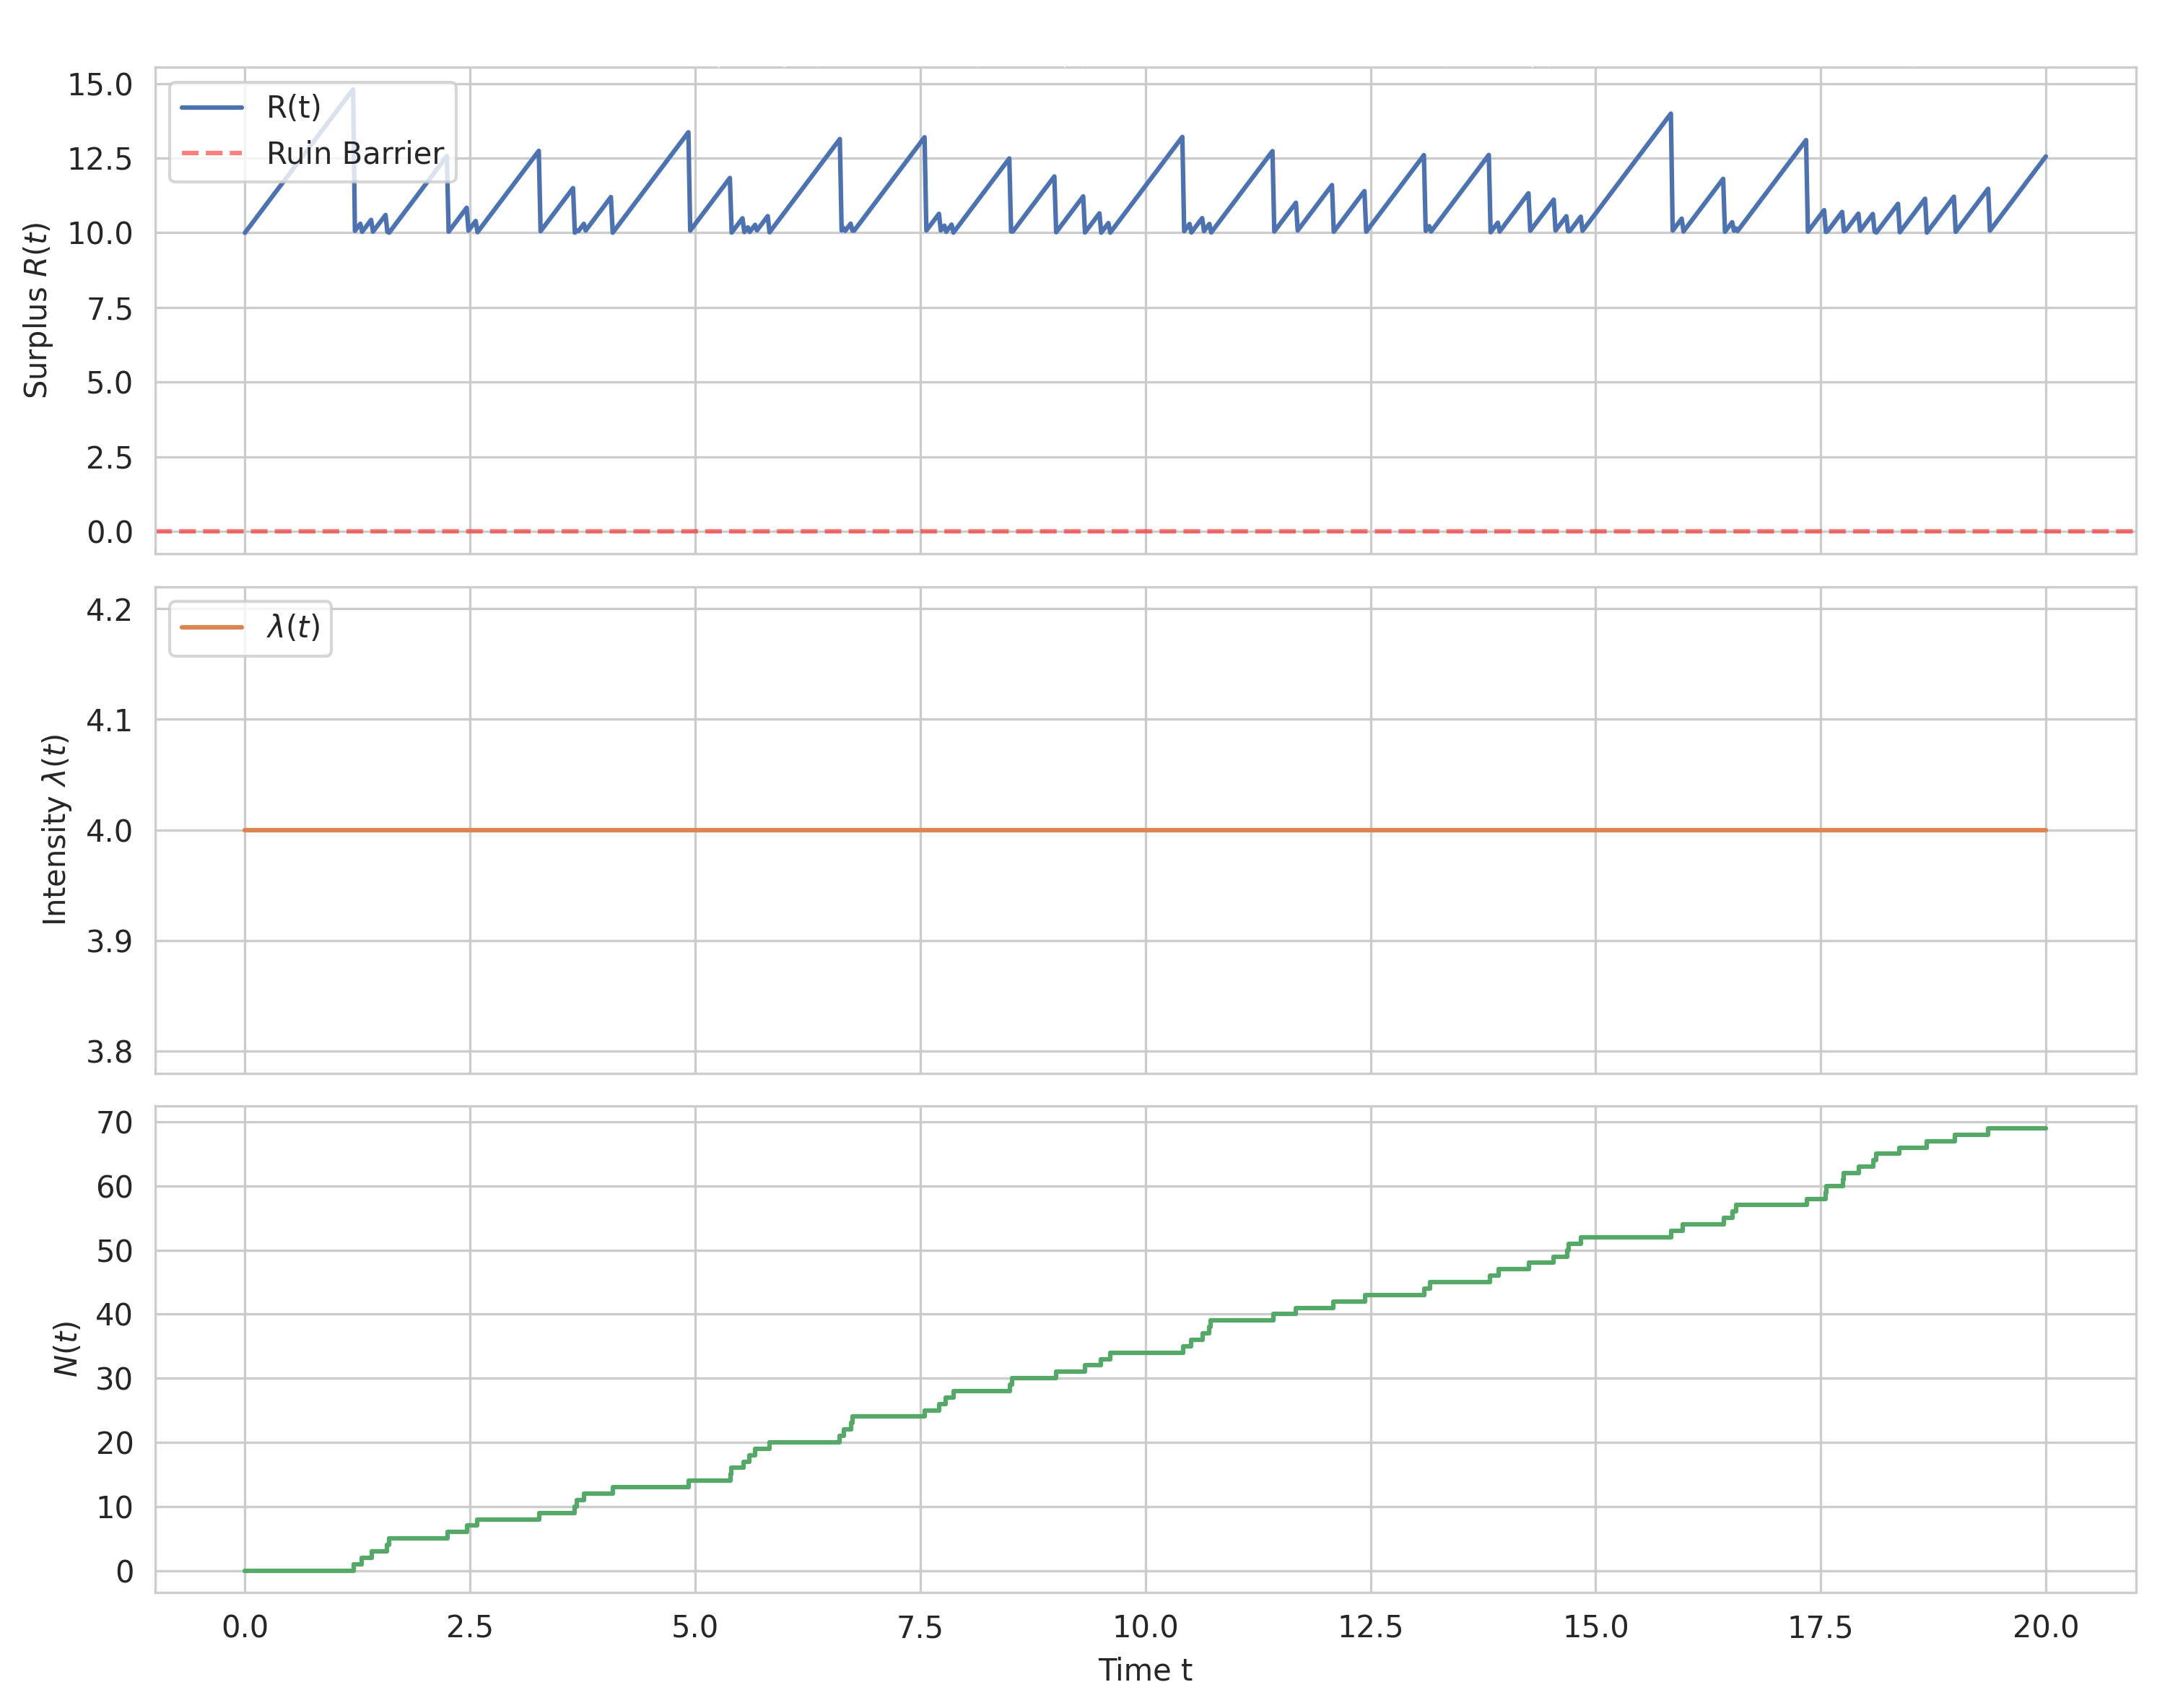
\includegraphics[width=\textwidth]{path_hpp.png}
        \caption{HPP}
    \end{subfigure}
    \hfill
    % --- IPP ---
    \begin{subfigure}{0.32\textwidth}
        \centering
        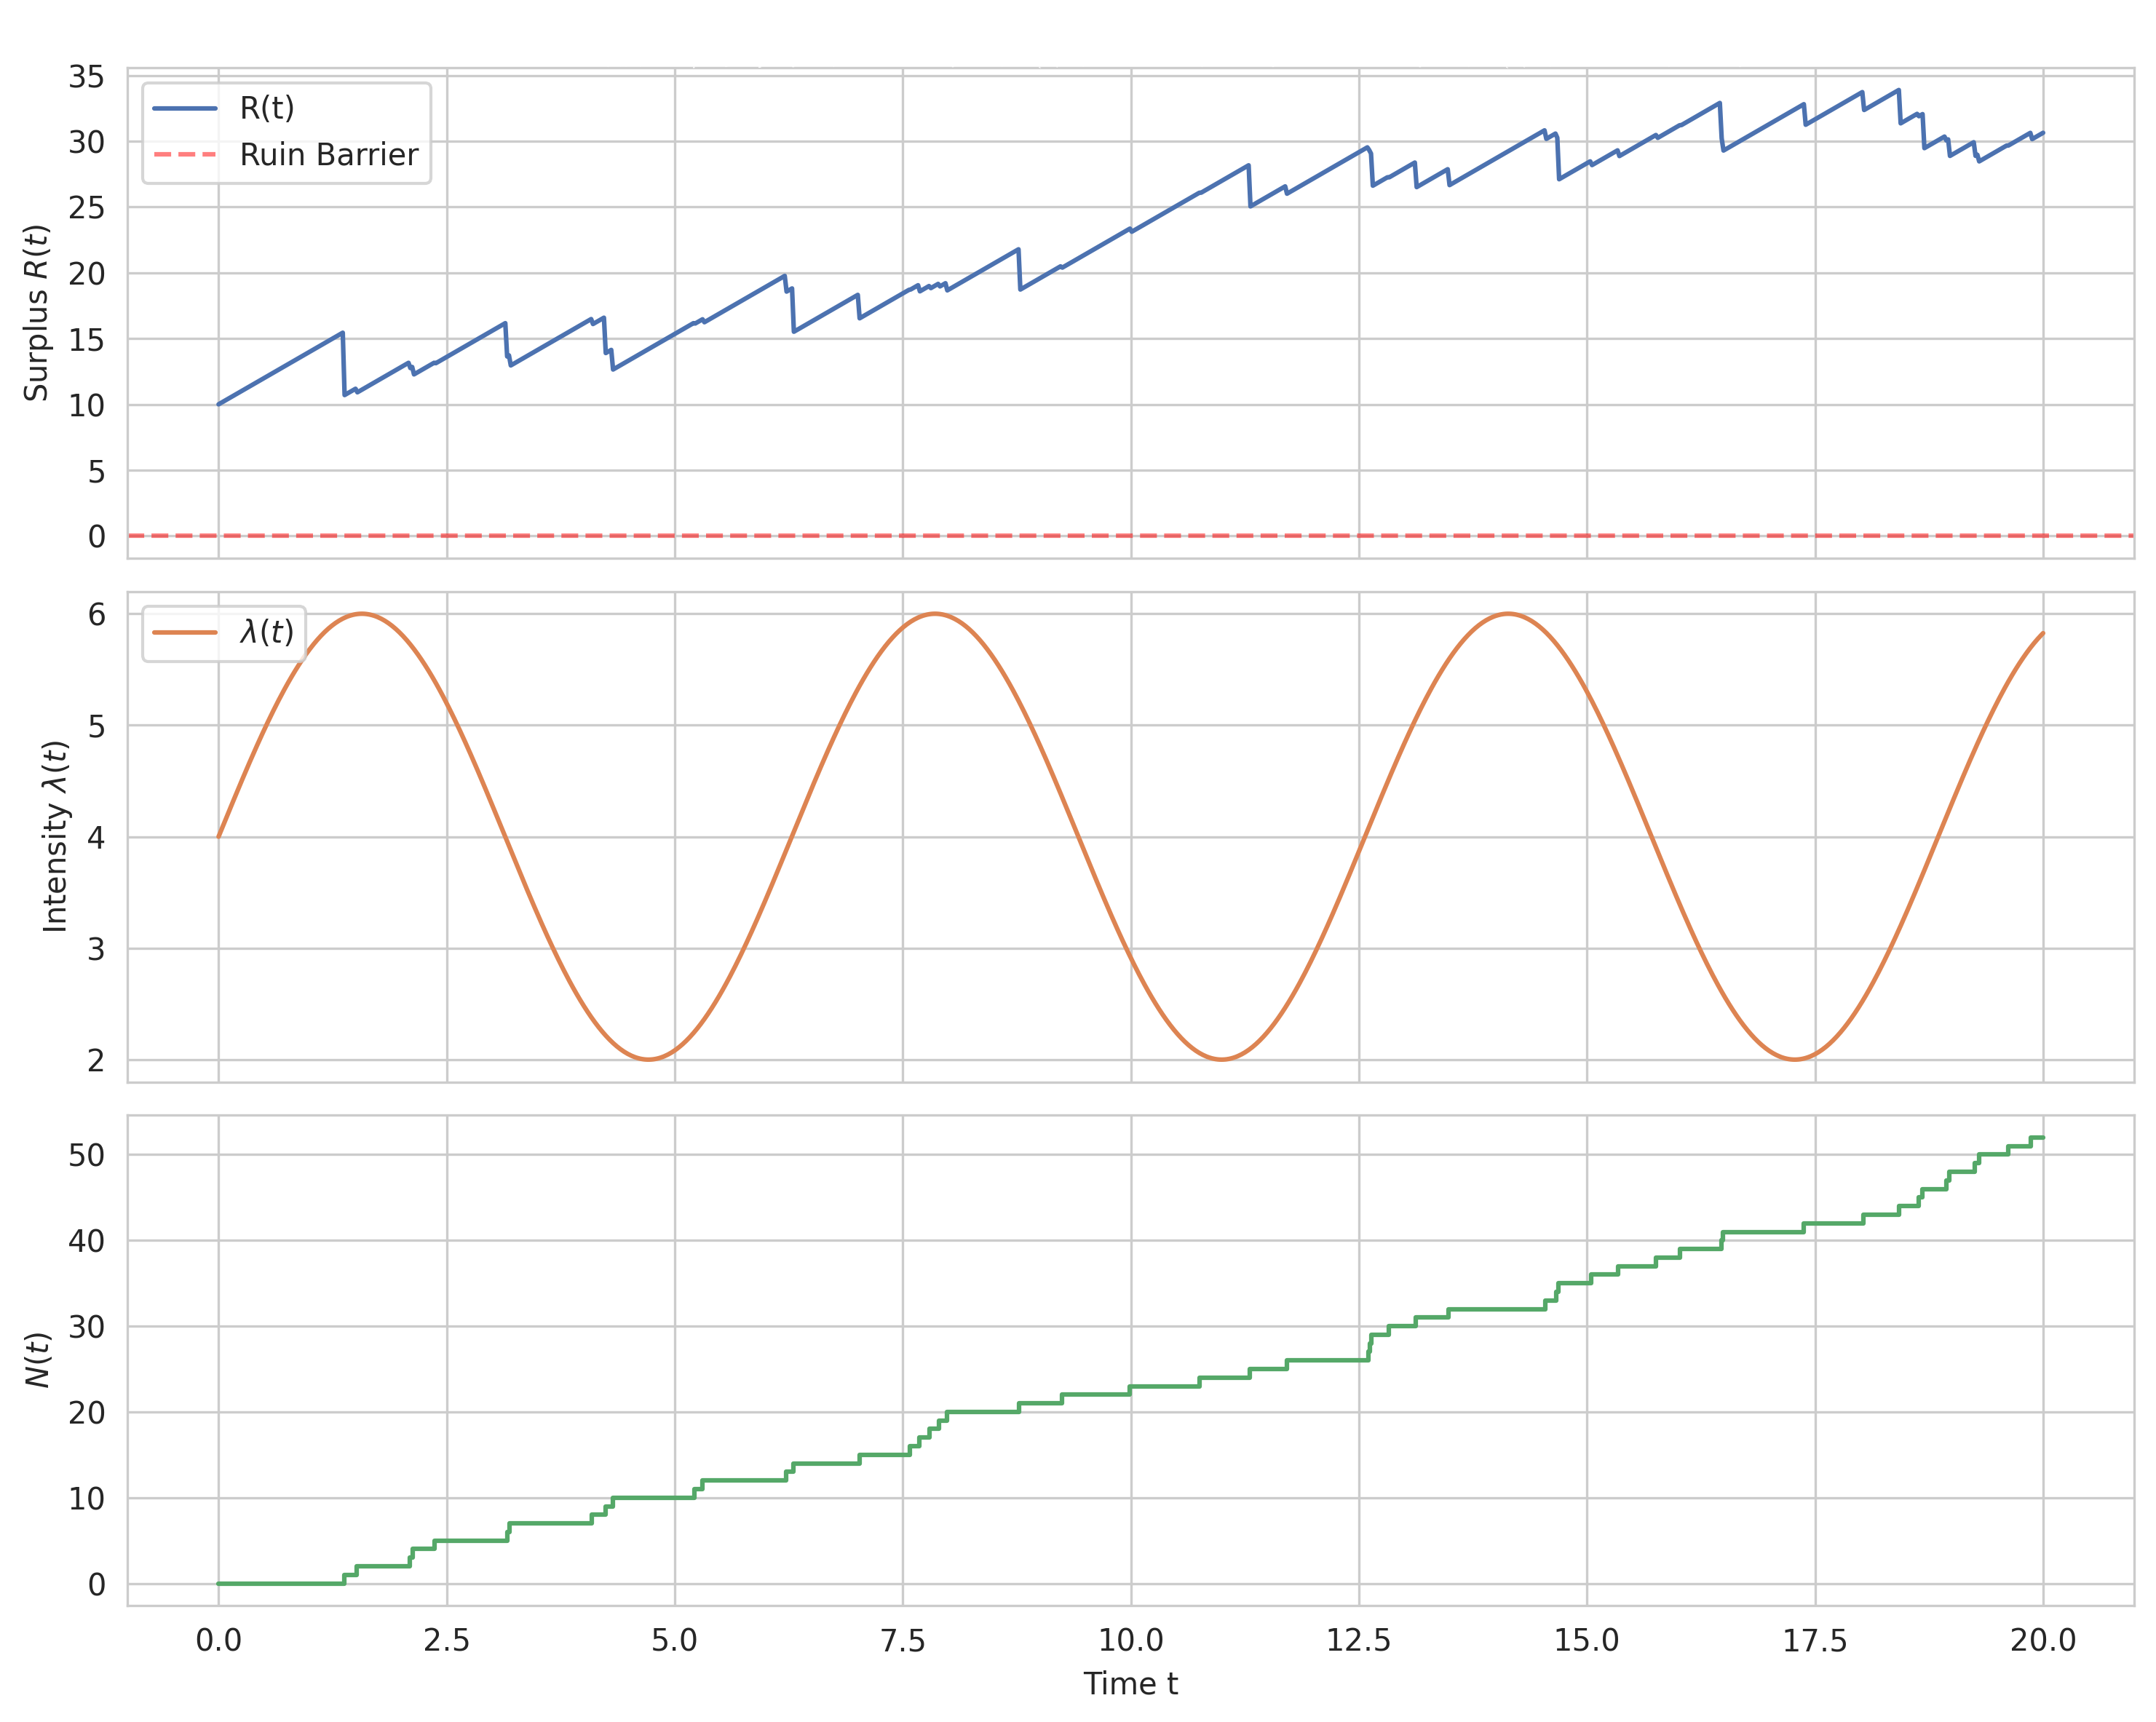
\includegraphics[width=\textwidth]{path_ipp.png}
        \caption{IPP}
    \end{subfigure}
    \hfill
    % --- Hawkes ---
    \begin{subfigure}{0.32\textwidth}
        \centering
        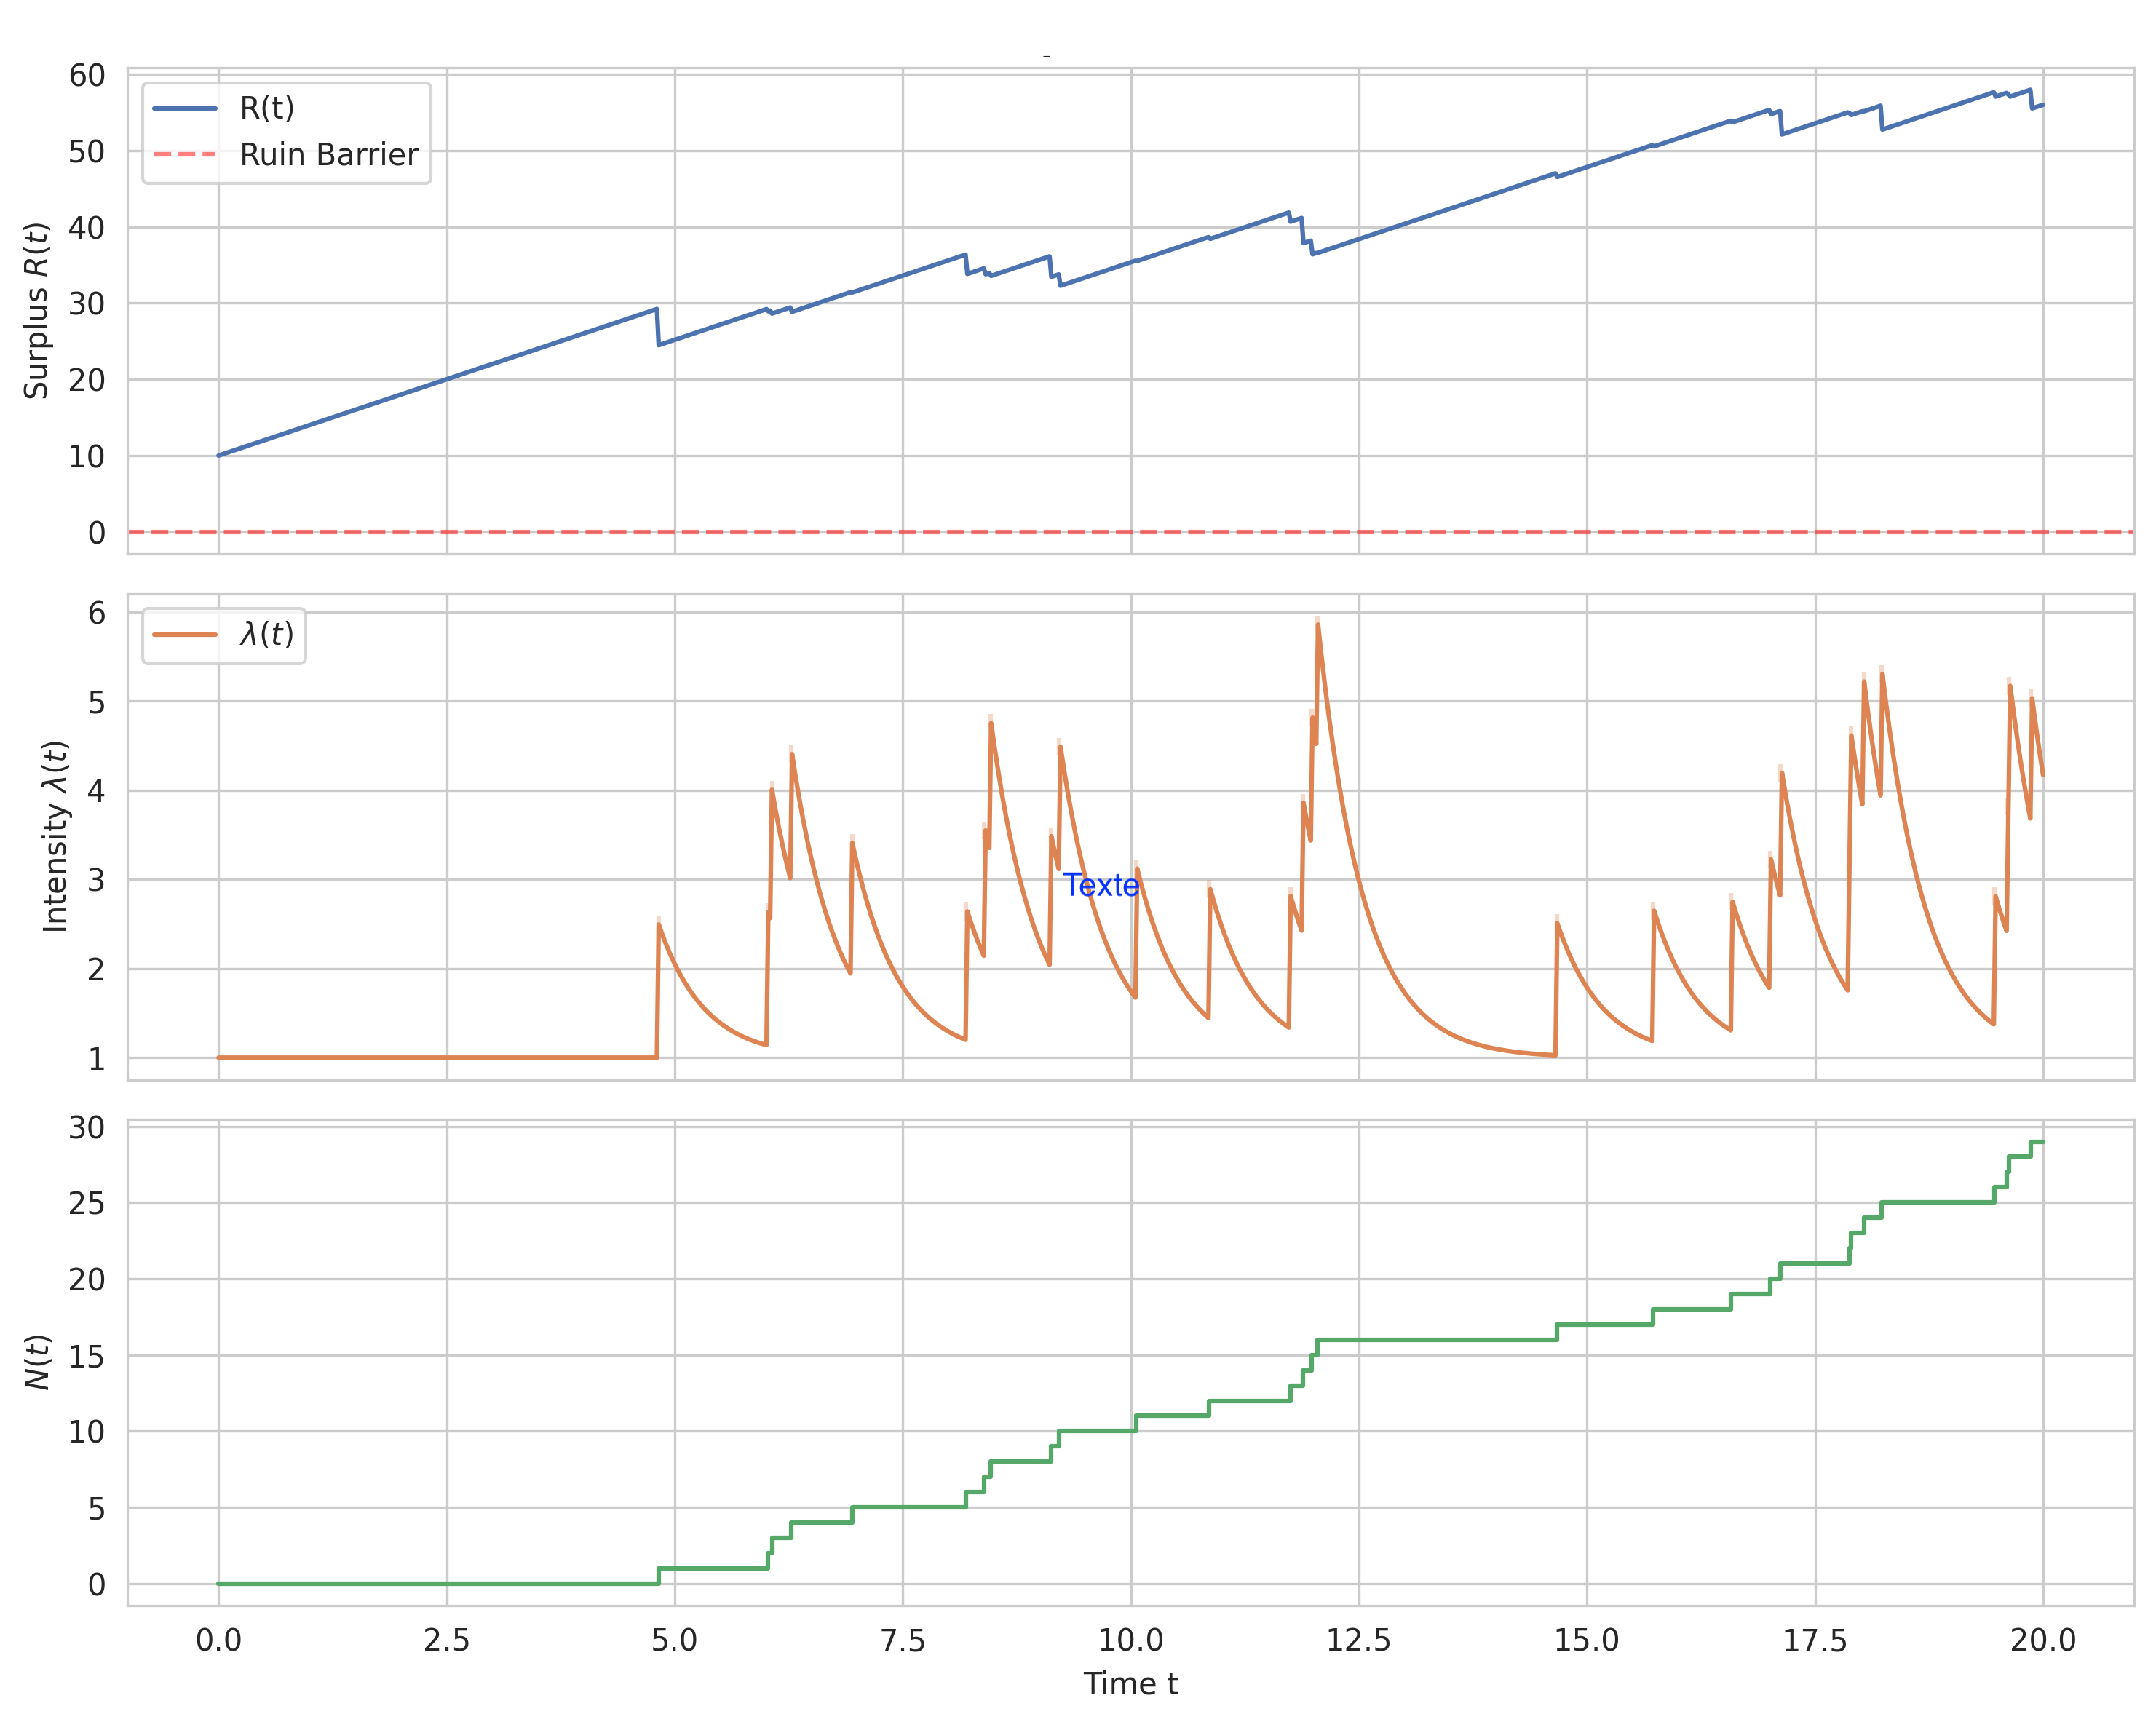
\includegraphics[width=\textwidth]{path_hawkes.png}
        \caption{Hawkes}
    \end{subfigure}

    \caption{\textbf{Comparison of intensity dynamics.}
    \text{Left:} Homogeneous Poisson Process — constant intensity. 
    \text{Middle:} Inhomogeneous Poisson Process — deterministic seasonal intensity. 
    \text{Right:} Hawkes process: self-exciting intensity with jumps after events and exponential decay, generating clustering and sharp drops in the surplus $R(t)$.}
    \label{fig:three_paths}
\end{figure}

\subsubsection*{Financial Calibration and Surplus Dynamics}
The evolution of the surplus process $R(t)$ is driven by the interaction between the premium income $ct$ and the claim flow $S(t)$. The parameters were calibrated as follows:
\begin{itemize}
    \item \textbf{Initial Capital ($u=10$):} Represents the starting solvency buffer. Without this endowment, the ruin would be immediate at the first cluster of claims.
    \item \textbf{Expected Profit (Drift):} We define the \textbf{drift} $d$ as the insurer's expected profit per unit of time: $d = c - \mathbb{E}[\lambda_{\infty}] \mathbb{E}[X] $
    In our simulation, with a premium rate $c=4.0$ and an expected loss of $4.0$ (Intensity $4.0 \times$ Mean Claim $1.0$), the theoretical drift is zero ($d=0$).
     \item \textbf{Analysis of Surplus Divergence: } Even if the theoritical drift of zero ($d=0$), the distinct upward trends observed in Figure 1 are the result of the discrepancy between the fixed premium rate (calibrated on the global mean) and the local instantaneous intensity.
  \begin{itemize}
    \renewcommand\labelitemii{$\bullet$}
    \item \textbf{HPP:} The risk is constant. As expected, the curve stays flat around the starting capital $u=10$.

    \item \textbf{IPP:} The curve goes up during "low seasons". We collect the same fixed premium, but pay fewer claims during these quiet times.

    \item \textbf{Hawkes:} This is the key visual effect. Between clusters, the intensity drops to a low baseline ($\lambda \approx 1$), but the premium is still calculated for a high average risk ($c=4$). The insurer effectively "makes money" during these quiet periods, building up reserves to survive the next cluster.
  \end{itemize}
\end{itemize}

\subsection{Quantifying the Cost of Clustering: A Comparison Between Hawkes and Poisson Models}

\subsubsection*{Ruin Probability: Hawkes vs. Poisson}

Figure \ref{fig:ruin_comparison} compares the probability of ruin under a Hawkes process and a homogeneous Poisson process, both calibrated to the same average intensity for different values of the premium rate c. 

The grey zone separates two zones : 

The vertical dotted line represents the minimal premium threshold $c_{min}$ required to satisfy the Net Profit Condition:
$$ c_{min} = \mathbb{E}[\lambda_{\infty}] \mathbb{E}[X]  = \frac{\mu}{1-n} \cdot \mathbb{E}[X] = \frac{0.5}{1-0.8}*1 = 2.5 $$ 

This axis separates the graph into two distinct regimes: on the left (Grey Zone), the condition is violated ($c < c_{min}$), and on the right (White Zone), it is verified ($c > c_{min}$).

    \textbf{Outside the grey zone ($c > c_{min}$):}  
    The net profit condition is verified, meaning the insurer makes an average profit. Consequently, the risk of ruin decreases rapidly as $c$ increases because the positive drift $d = c - \mathbb{E}[\lambda_{\infty}] \mathbb{E}[X]$ pulls the capital away from zero.
    However, for the \textbf{Hawkes process}, this drop is significantly slower (the red curve stays above the blue one). Even with a positive drift, the "clustering effect" creates sudden, deep drawdowns that can breach the solvency barrier where the smoother Poisson process would survive.

    \textbf{Inside the grey zone ($c < c_{min}$):}  
    The net profit condition is not verified. Cumulative gains are strictly less than cumulative losses, making ruin mathematically certain over an infinite horizon ($\psi(u) = 1$).\\
    However, our simulation is over a \textbf{finite time horizon}. 
    The Hawkes process (Red) shows a \textit{lower} ruin probability than Poisson (Blue) here.
    Between clusters, the Hawkes intensity drops to its baseline ($\mu < \lambda_{Poisson}$), meaning the insurer loses money \textit{slower} than in the Poisson model during these quiet periods. This delays the time of ruin, allowing some trajectories to "survive" until the end of the simulation simply because the fatal cluster didn't arrive yet.

\begin{figure}[H]
    \centering
    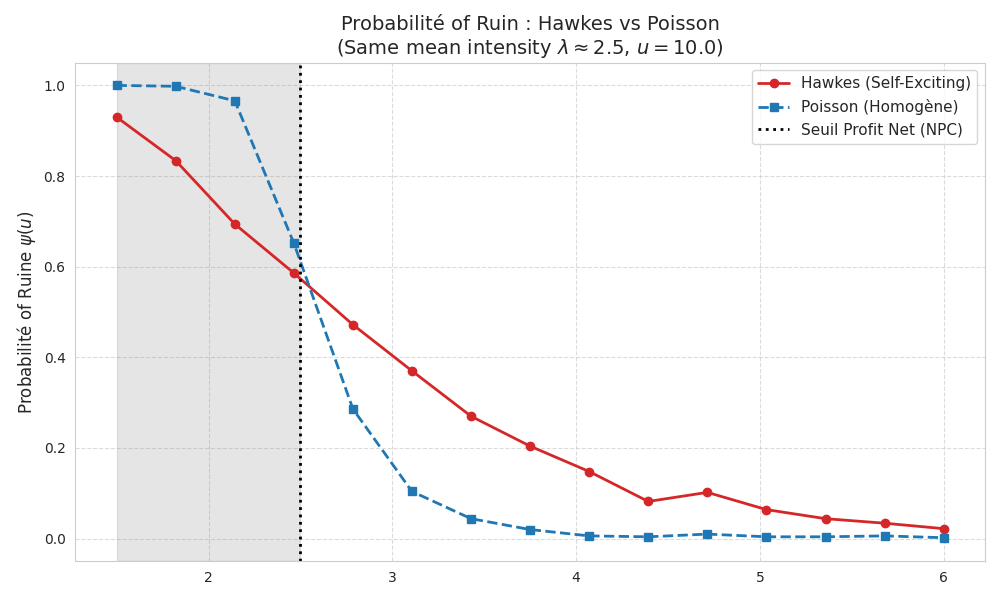
\includegraphics[width=0.6\textwidth]{ruin_hawkes_vs_poisson.png}
    \caption{\textbf{Probability of ruin $\psi(u)$ as a function of the premium rate $c$.} 
    Results are estimated using 500 Monte Carlo simulations over a time horizon $T=100$.
    Both models share the same average intensity $\lambda \approx \lambda_{eq}$ and initial capital $u$.
    The vertical dotted line represents the Net Profit Condition (NPC) threshold. 
    The shaded region corresponds to the regime where the NPC is violated, leading to almost certain ruin. 
    The Hawkes process exhibits systematically higher ruin probabilities due to the clustering effect.}
    \label{fig:ruin_comparison}
\end{figure}

\subsubsection*{Comparison of Three Self-Exciting Regimes}

Figure \ref{fig:ruin_regimes} illustrates the impact of three different self-exciting regimes on the probability of ruin, while keeping the average intensity constant at $\lambda = \lambda_{\text{target}}$. While, critical self-excitation regime increases the clustering effect and the probability of ruin. 
\\
\textbf{Non-Solvent Zone ($c < c_{min}$):}
Paradoxically, the Critical Regime ($n^*=0.9$, Red) appears safer. To maintain the average intensity, its baseline $\mu$ is set very low. Consequently, long "quiet periods" delay the time of ruin, whereas the Low Regime drains capital continuously like a Poisson process.
\\
\textbf{Solvent Zone ($c > c_{min}$):}
The Critical Regime remains dangerous even with high premiums ($c=5.0$). Due to "heavy tails," a single massive cluster can still wipe out the capital. Simply increasing the premium rate is ineffective against this structural risk.
\begin{figure}[H]
    \centering
    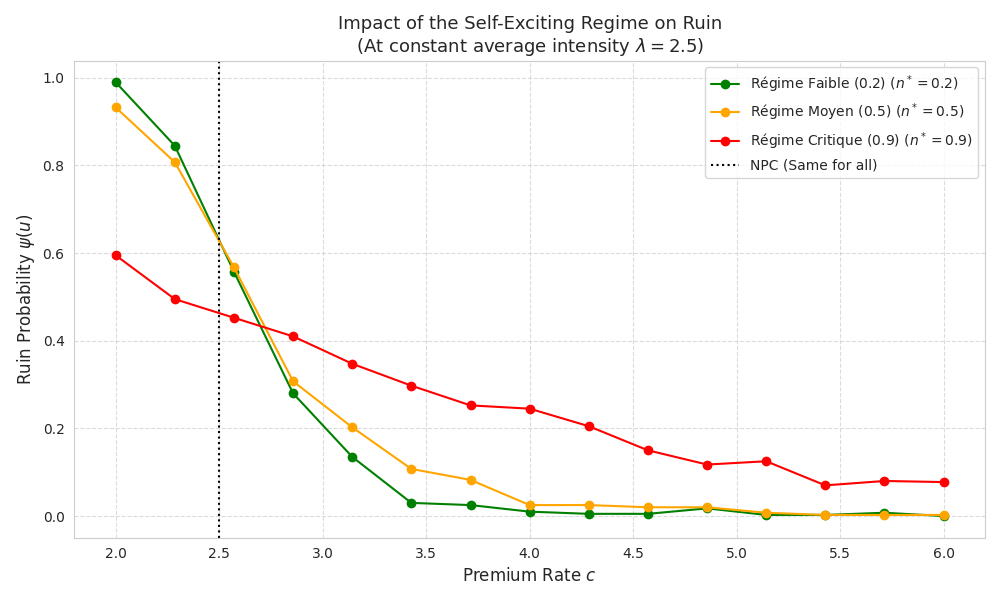
\includegraphics[width=0.6\textwidth]{regimes.png}
    \caption{\textbf{Probability of ruin under three self-exciting regimes.} 
    The x-axis represents the premium rate $c$, and the y-axis shows the ruin probability $\psi(u)$. 
    The vertical dotted line indicates the Net Profit Condition (NPC), which is identical for all regimes. 
    The three curves correspond to low ($n^*=0.2$), medium ($n^*=0.5$), and critical ($n^*=0.9$) self-excitation regimes. 
    Higher self-excitation leads to systematically higher ruin probabilities, even though the average intensity $\lambda$ is the same.}
    \label{fig:ruin_regimes}
\end{figure}

\subsubsection*{Sensitivity to the Initial Capital}

Figure \ref{fig:ruin_vs_u} shows the impact of the initial capital $u$ on the probability of ruin for both Hawkes and Poisson risk processes, using a fixed premium rate $c=3.5 > \text{NPC}$. 

In insurance context, the Solvency Capital Requirement (SCR) is defined as the minimum initial capital required to maintain the ruin probability below a specific tolerance threshold, typically set at 5\%. Figure 4 illustrates a significant disparity between the two models. For the Poisson process, the SCR is approximately $u \approx 9$, which represents roughly 2.5 times the premium rate ($c$). In contrast, for the Hawkes process, extrapolating the curve suggests that the SCR would exceed $u = 50$ or $60$, corresponding to 15 to 17 times the premium rate.This comparison demonstrates that managing self-exciting risks solely through equity capital is economically inefficient. Consequently, it is necessary to either increase the premium rate $c$ (as analyzed in Figure 3) or to use reinsurance strategies (as discussed in Figure 6).

\begin{figure}[H]
    \centering
    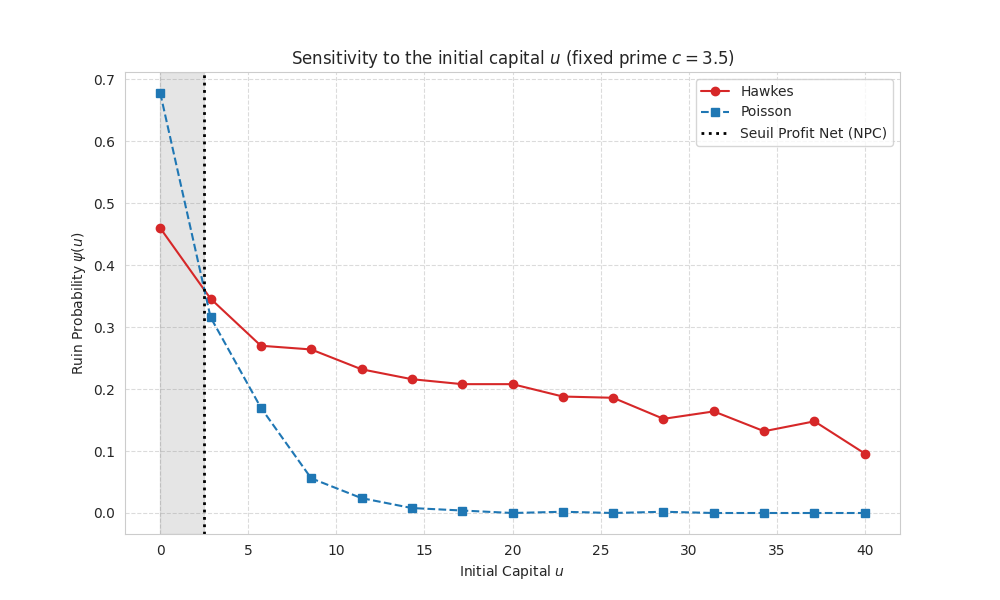
\includegraphics[width=0.6\textwidth]{Influence_of_u_on_Ruin.png}
    \caption{\textbf{Ruin probability as a function of the initial capital $u$.}
    The premium rate is fixed at $c = 3.5$, ensuring a profitable regime ($c>\text{NPC}$). 
    The Hawkes model consistently exhibits higher ruin probabilities due to claim clustering. 
    The decay of the curves illustrates the classical Lundberg-type exponential behavior.}
    \label{fig:ruin_vs_u}
\end{figure}

\subsection{Model Risk and Sensitivity Analysis to Parameter Estimation Errors}

To simulate a Hawkes process, we essentially need to calibrate two main parameters: $\alpha$ (which controls the jump intensity) and $\beta$ (which controls the memory decay). Usually, we use Maximum Likelihood Estimation (MLE) for this. 

However, in practice, this calibration is extremely difficult. The likelihood function can be very flat, meaning that different pairs of parameters can fit the data almost equally well. This leads to a significant "Model Risk."

Since the stability of the process depends on the branching ratio $n = \alpha / \beta$, it is more interesting to fix one parameter and vary the other to see the impact. Here, we fixed $\beta = 1$ and introduced an estimation error on $\alpha$ ranging from $-10\%$ to $+10\%$.

As shown in Figure \ref{fig:Calibration_error}, the results are striking:

\begin{itemize}
    \item \textbf{The Blue Curve (Stable Regime, $n^*=0.65$):} The model is quite robust. Even with calibration errors, the probability of ruin stays flat and low.
    
    \item \textbf{The Red Curve (Critical Regime, $n^* \approx 0.80 - 0.90$):} Here, the model becomes extremely sensitive. We can see that a simple $10\%$ positive error in the estimation of $\alpha$ causes the probability of ruin to jump from $0.1$ to nearly $0.7$.
\end{itemize}


\begin{figure}[H]
    \centering
    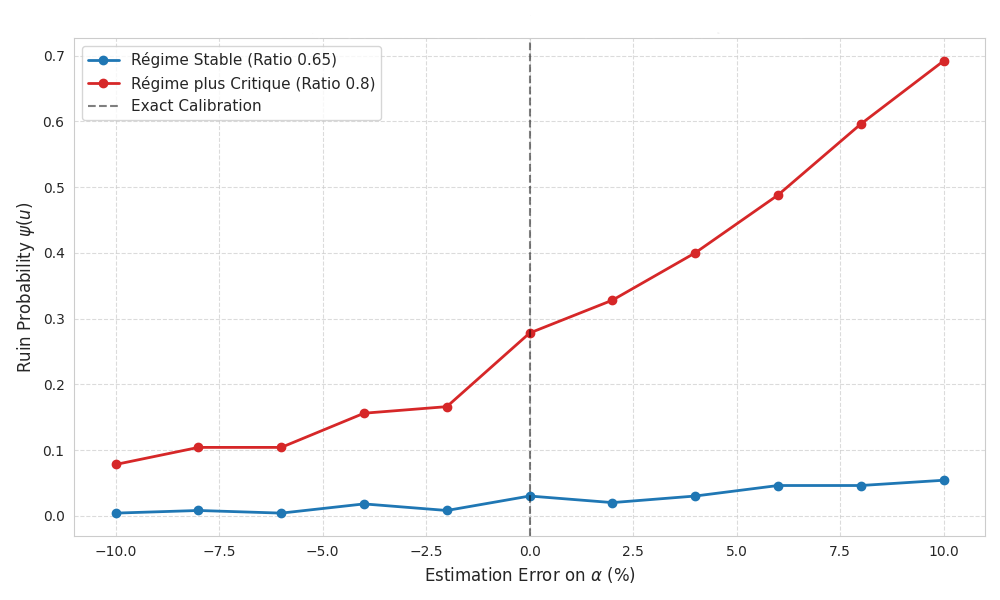
\includegraphics[width=0.6\textwidth]{images/Calibration_error.png}
    \caption{\textbf{Impact of a 10\% calibration error on the probability of ruin.} 
    The curves correspond to two self-exciting regimes: a stable regime ($n^*=0.65$) and a critical regime ($n^*=0.90$). 
    The x-axis represents the estimation error applied to the self-excitation parameter $\alpha$, while the y-axis shows the resulting ruin probability $\psi(u)$. 
    The vertical dashed line marks the exact calibration. 
    The results highlight the high sensitivity of the critical regime to miscalibration, where even small positive errors can lead to a sharp increase in ruin probability, whereas the stable regime exhibits a more moderate response.}
    \label{fig:Calibration_error}
\end{figure}


\subsection*{Why does this happen?}

Mathematically, this explosion is due to the formula of the expected intensity. The long-term expectation depends on the multiplier $\frac{1}{1-n}$:
\begin{equation}
    E[\lambda(t)] = \frac{\mu}{1 - n}
\end{equation}
When we are in a critical regime (where $n$ is close to 1), a small error on $\alpha$ pushes $n$ even closer to 1. This causes the denominator $(1-n)$ to vanish, making the expected loss (and thus the ruin probability) explode exponentially.

\textbf{Conclusion:} In a critical regime, we cannot rely solely on the model's calibration, because a tiny error can lead to a massive underestimation of the risk. This motivates the need for an external protection mechanism, such as the Stop Loss reinsurance studied in the next part.

\subsection{Risk Mitigation Strategies: Stop-Loss Reinsurance}

\subsection*{Mathematical Framework: The Stop-Loss Treaty}
To mitigate the high risk of ruin induced by the self-exciting nature of the Hawkes process, we implemented a reinsurance strategy known as \textbf{Stop-Loss}. 

Let $S_t$ be the aggregate claim amount for year $t$, defined as the sum of all individual claims occurring in that year. The reinsurance treaty is defined by a retention limit (or priority) $P$. The amounts paid by the insurer ($I_t$) and the reinsurer ($R_t$) are given by:
\begin{equation}
    \begin{aligned}
        I_t &= \min(S_t, P) \\
        R_t &= (S_t - P)^+ = \max(0, S_t - P)
    \end{aligned}
\end{equation}

The insurer is thus fully protected against annual losses exceeding $P$. In exchange for this protection, the insurer pays a reinsurance premium $\Pi_{re}$, reducing its net annual income. Consequently, the net surplus dynamic $R(t)$ evolves according to the following recursive equation:
\begin{equation}
    R(t) = R(t-1) + \Pi_{gross} - \Pi_{re} - \min(S_t, P)
\end{equation}
Where:
\begin{itemize}
    \item $R(t-1)$ is the available capital at the start of the year;
    \item $\Pi_{gross}$ is the total premium collected from policyholders;
    \item $\Pi_{re}$ is the cost of the Stop-Loss treaty.
\end{itemize}


\subsection*{Calibration of the Treaty}
For our simulation, the treaty was calibrated to act as a \textit{"Catastrophe Shield"}. The parameters were set as follows:
\begin{itemize}
    \item \textbf{Priority ($P$):} Fixed at $120\%$ of the average annual loss. This means the insurer handles the \textbf{normal variations} in claims (day-to-day accidents), while transferring the risk of \textbf{extreme accumulations} (when claims pile up rapidly) to the reinsurer.
    \item \textbf{Reinsurance Cost:} The price of protection $\Pi_{re}$ was set to $20\%$ of the gross premium. This substantial cost reduces the net drift (average capital growth) but is the necessary trade-off to secure the insurer's solvency.
\end{itemize}
\subsection*{Empirical Analysis}
Figure~\ref{fig:reinsurance_critical} compares the capital evolution and ruin probabilities between the \textbf{Gross strategy} (without reinsurance, in blue) and the \textbf{Net strategy} (with Stop-Loss, in green) under a critical Hawkes regime ($n^*=0.8$).

\begin{figure}[htbp]
    \centering
    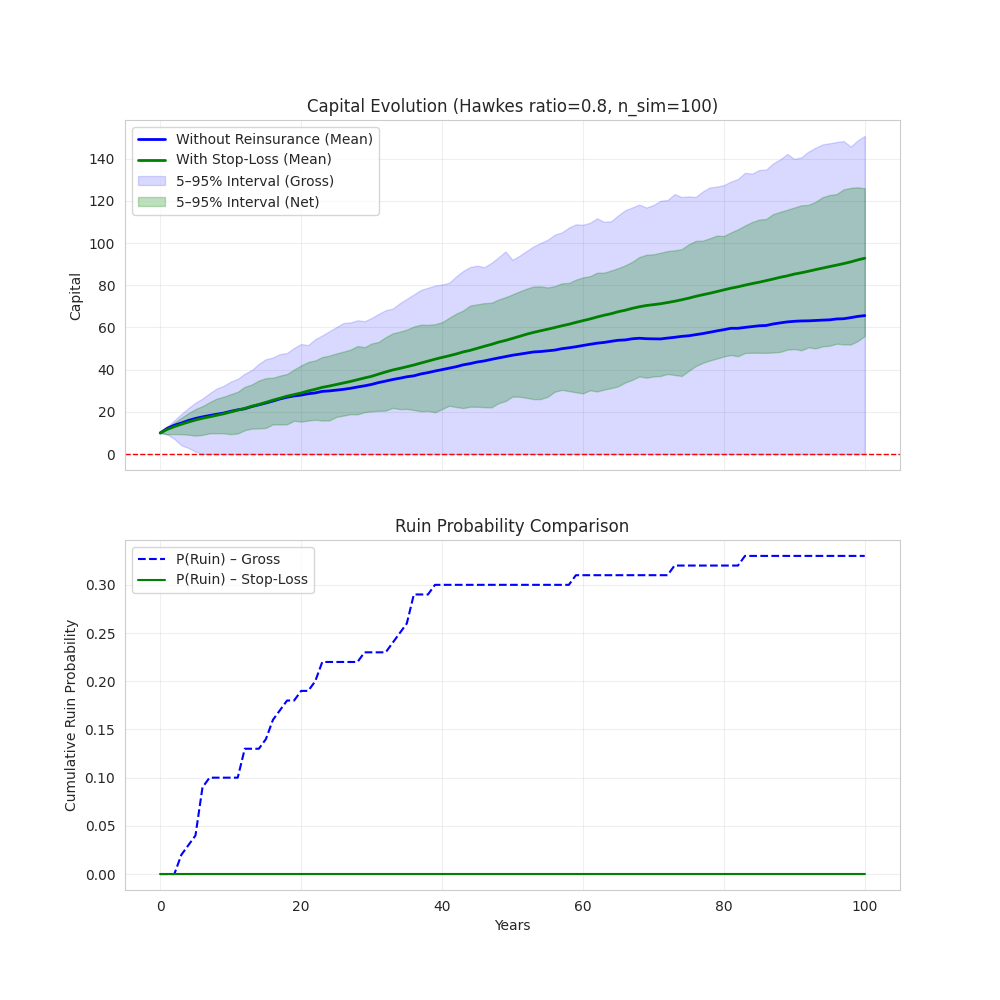
\includegraphics[width=0.7\textwidth]{reinsurance.png}
    \\
\caption{\textbf{Impact of Stop-Loss reinsurance under a critical Hawkes regime ($n^*=0.8$).} 
    The simulation compares the Gross strategy (Blue) vs. the Net strategy with Stop-Loss (Green).
    \text{(a) Capital Evolution:} The Blue area is very wide and unstable, showing that without reinsurance, the capital often drops dangerously close to zero. The Green area is much narrower: despite paying $20\%$ of the premiums for reinsurance, the capital grows steadily and stays safe.
    \text{(b) Cumulative Ruin Probability:} Without reinsurance (Blue line), the risk of bankruptcy rises to $\approx 35\%$ due to sudden clusters of claims. With Stop-Loss (Green line), this risk is eliminated ($0\%$), as the reinsurance absorbs the shock of extreme events.}
    \label{fig:reinsurance_critical}
\end{figure}


\clearpage
\section*{Conclusion}
\addcontentsline{toc}{section}{Conclusion}

In this report, we explored a variation of the Cramér-Lundberg model which enabled us to visualize the impact of self-excitation on insurance risk. By using the Hawkes process as our claim counting process, we were able to capture the phenomenon of claim clustering, which seems to be closer to many real-world insurance scenarios.

Our theoretical analysis established the exact expression for the expected number of claims and derived the resulting NPC. We demonstrated that the stability of the portfolio relies heavily on the branching ratio $n = \alpha / \beta$. While the NPC provides a necessary lower bound for premiums, our simulations revealed that it is usually not enough to guarantee profitability in the short term.

Through Monte Carlo simulations, using Ogata’s thinning algorithm, we quantified the specific cost of clustering. Our analysis yielded several key findings:
\begin{itemize}
    \item \textbf{Underestimation of Risk:} For an equivalent average claim frequency, the Hawkes process generates a significantly higher probability of ruin than both homogeneous and inhomogeneous Poisson processes. Frequently, the temporal concentration of claims leads to capital decreasing faster than premiums can be collected.
    \item \textbf{Capital Inefficiency:} We observed that relying solely on initial capital to reduce self-exciting risks is economically inefficient. The Solvency Capital Requirement (SCR) increases non-linearly with the excitation parameter $\alpha$, requiring larger reserves for higher clustering regimes.
    \item \textbf{Model Risk:} We highlighted the extreme sensitivity of the model to parameter estimation errors. In high-excitation regimes ($n \to 1$), a minor calibration error can lead to a drastic underestimation of the ruin probability.
\end{itemize}

Finally, we explored risk mitigation strategies and showed that Stop-Loss reinsurance acts as an effective stabilizer. By transferring the tail risk associated with extreme clusters to a reinsurer, the primary insurer can maintain capital stability and reduce the probability of ruin.


\begin{thebibliography}{9}
\bibitem{hawkes1974}
A. G. Hawkes and D. Oakes, ``A cluster process representation of a self-exciting process,'' \textit{Journal of Applied Probability}, vol. 11, no. 3, pp. 493--503, 1974.

\bibitem{bacry2015}
E. Bacry, I. Mastromatteo, and J.-F. Muzy, ``Hawkes processes in finance,'' \textit{Market Microstructure and Liquidity}, vol. 1, no. 01, 2015.

\bibitem{ogata1981}
Y. Ogata, ``On Lewis' simulation method for point processes,'' \textit{IEEE Transactions on Information Theory}, vol. 27, no. 1, pp. 23--31, 1981.
\end{thebibliography}


\clearpage
\appendix

\section*{Appendix} 
\addcontentsline{toc}{section}{Appendix} 

\section{Proof of the expectation value of a Hawkes process with an exponential kernel}

Our objective is to derive the expression for the expected number of events $\mathbb{E}[N(t)]$ for a Hawkes process with an exponential kernel.

The expected number of events up to time $t$ is given by the integral of the mean intensity
$$     \mathbb{E}[N(t)] = \mathbb{E}\left[ \int_0^t \lambda(s) ds \right]
$$ 
Assuming that $\mathbb{E}[\lambda(t)] < \infty$ for all $t \ge 0$, we can apply Fubini's theorem
$$ 
\mathbb{E}[N(t)] = \int_0^t \mathbb{E}[\lambda(s)] ds
$$ 
Using the definition of the Hawkes process intensity
$$     \mathbb{E}[N(t)] = \int_0^t \left( \mu + \int_0^s \phi(s - x) \mathbb{E}[dN(x)] \right) ds
$$ 
Let $m(t) = \mathbb{E}[N(t)]$. Differentiating with respect to $t$
$$     m'(t) = \mu + \int_0^t \phi(t - x) m'(x) dx
$$ 
We apply the Laplace transform $\tilde{f}(p) = \int_0^\infty e^{-pt} f(t) dt$ to both sides
$$    \tilde{m'}(p) = \frac{\mu}{p} + \tilde{\phi}(p) \tilde{m'}(p)
$$
$$     \tilde{m'}(p) = \frac{\mu}{p(1 - \tilde{\phi}(p))}
$$ 
As referenced in \cite{bacry2015}, the finiteness of $\mathbb{E}[N(t)]$ requires the stability condition $n  = \tilde{\phi}(0) < 1$.

For the exponential kernel $\phi(t) = \alpha e^{-\beta t}$, the Laplace transform is:
$$     \tilde{\phi}(p) = \frac{\alpha}{p + \beta}
$$ 
The stability condition implies $\tilde{\phi}(0) = \frac{\alpha}{\beta} < 1$, i.e., $\alpha < \beta$. Substituting this into the expression for $\tilde{m'}(p)$
$$    \tilde{m'}(p) = \frac{\mu}{p \left(1 - \frac{\alpha}{p + \beta}\right)} = \frac{\mu (p + \beta)}{p (p + \beta - \alpha)}
$$*
Using partial fraction decomposition and taking the inverse Laplace transform, we find the closed-form expression for the mean intensity $m'(t) = \mathbb{E}[\lambda(t)]$
$$    m'(t) = \frac{\mu}{\beta - \alpha} \left(\beta - \alpha e^{-(\beta - \alpha) t}\right)
$$
Finally, by integrating
\begin{equation}
    \boxed{m(t) = \frac{\mu}{\beta - \alpha} \left( \beta t - \frac{\alpha}{\beta - \alpha} (1 - e^{-(\beta - \alpha) t}) \right)}
\end{equation}

\section{Proof by Induction}

Let $n$ denote the average number of direct events generated by a single excitation.

Let $Z_k$ be the random variable representing the number of events at generation $k$ coming from a single immigrant. We want to show that
\begin{equation}
    \mathbb{E}[Z_k] = n^k
\end{equation}

\textbf{Base Case ($k=0$):}
By definition, we start with a single immigrant, so $Z_0 = 1$.
$$ \mathbb{E}[Z_0] = 1 = n^0 $$
The property holds for $k=0$.

\textbf{Inductive Step:}
Assume $\mathbb{E}[Z_k] = n^k$. The number of events at generation $k+1$ is the sum of the direct descendants generated by the $Z_k$ events of the previous generation. Let $X_i$ denote the number of descendants from the i-th event of generation $k$, where $\mathbb{E}[X_i] = n$. We have:
$$ Z_{k+1} = \sum_{i=1}^{Z_k} X_i $$
Using Wald's identity (since $Z_k$ is independent of the descendants counts $X_i$), we obtain:
$$ \mathbb{E}[Z_{k+1}] = \mathbb{E}[Z_k] \cdot \mathbb{E}[X_i] $$
Using the inductive hypothesis:
$$ \mathbb{E}[Z_{k+1}] = n^k \cdot n = n^{k+1} $$

\textbf{Conclusion:}
The property holds for all $k \ge 0$.

\end{document}